\documentclass[
  a4paper,
  abstract=true,
  twoside,
  listof=totoc,
  numbers=noenddot,
  bibliography=totoc,
  BCOR1.5cm,
  % headsepline,
  DIV12,
  %appendixprefix,
  final,
  %fontsize=10pt,
  openany
] {scrbook}

\iffalse
% book margin fix: http://www.khirevich.com/latex/page_layout/
\makeatletter
\if@twoside % commands below work only for twoside option of \documentclass
    \newlength{\textblockoffset}
    \setlength{\textblockoffset}{12mm}
    \addtolength{\hoffset}{\textblockoffset}
    \addtolength{\evensidemargin}{-2.0\textblockoffset}
\fi
\makeatother
\fi


% You should select either american or british instead of english here:
\usepackage[american]{babel}
%\usepackage{fontspec}
\usepackage{amsmath}
\usepackage{appendix}
\usepackage{listings}
\usepackage[pdftex,
citebordercolor={0.75 0.75 1},
filebordercolor={0.75 0.75 1},
linkbordercolor={0.75 0.75 1},
% pagebordercolor={0.75 0.75 1},
urlbordercolor={0.75 0.75 1},
pdfborder={0.75 0.75 1},plainpages=false,pdfpagelabels=true]{hyperref}
\hypersetup{%
  pdftitle={MSc DSE Thesis: An Integrity Protected File System Layer for Intel SGX},
  pdfauthor={Prateek Bhatnagar},
  pdfkeywords={Master of Science, Thesis, Distributed Systems Engineering},
}

\usepackage[backend=biber,style=numeric,alldates=long]{biblatex}
% \usepackage[backend=biber,style=alphabetic,alldates=long]{biblatex}

% \usepackage{luatex85}
\usepackage{pdfpages}
\usepackage{color}
\usepackage{varioref}           % nice refs
\usepackage{csquotes}
\usepackage{graphicx}           % graphics
\usepackage{caption}            % manipulate fugures
\usepackage{subcaption}         % allow for subfigures
\usepackage{listings}           % nice source code listings
\usepackage{booktabs}           % nice tables
\usepackage{microtype}          % better looking text borders
\usepackage{units}              % unified way of setting values with units
\usepackage{array}
\usepackage{fancybox}           % provide nice boxes
\usepackage{fancyvrb}           % algorithm-boxes
\usepackage{xspace}
\usepackage{setspace}
\usepackage{hyphenat}
\usepackage{todonotes}
\usepackage[acronym,shortcuts]{glossaries}
\usepackage{svg}
\usepackage[T1]{fontenc}
\usepackage{csvsimple}
\usepackage{diagbox}
\usepackage{pifont}
\usepackage{multirow}

% use this one last
% (redefines some macros for compatibility with KOMAScript)
\usepackage{scrhack}



\definecolor{mygreen}{rgb}{0,0.6,0}
\definecolor{mygray}{rgb}{0.5,0.5,0.5}
\definecolor{mymauve}{rgb}{0.58,0,0.82}

\definecolor{fblue}{RGB}{92,144,192}
\definecolor{fgreen}{RGB}{34,162,70}

%  D5E8D4
\definecolor{drawio_light_green}{rgb}{213,232,212}



% Biblatex Style
\setcounter{secnumdepth}{4}     % limit enumeration depth
\setcounter{tocdepth}{2}        % limit TOC depth

% Listing Style

\lstset{ %
  frame=shadowbox,
  rulesepcolor=\color{white},
  backgroundcolor=\color{white},   % choose the background color; you must add \usepackage{color} or \usepackage{xcolor}
  basicstyle={\footnotesize\ttfamily},        % the size of the fonts that are used for the code
  breakatwhitespace=false,         % sets if automatic breaks should only happen at whitespace
  breaklines=true,                 % sets automatic line breaking
  captionpos=b,                    % sets the caption-position to bottom
  commentstyle=\color{mygreen},    % comment style
  deletekeywords={...},            % if you want to delete keywords from the given language
  escapeinside={\%*}{*)},          % if you want to add LaTeX within your code
  extendedchars=true,              % lets you use non-ASCII characters; for 8-bits encodings only, does not work with UTF-8
  frame=L,                    % adds a frame around the code
  frameround=tttt,
  keepspaces=true,                 % keeps spaces in text, useful for keeping indentation of code (possibly needs columns=flexible)
  keywordstyle=\color{blue},       % keyword style
  language=bash,                 % the language of the code
  morekeywords={scone, fspf, git,* __thread, bool, false, true},            % if you want to add more keywords to the set
  numbers=left,                    % where to put the line-numbers; possible values are (none, left, right)
  numbersep=7pt,                   % how far the line-numbers are from the code
  numberstyle=\color{mygray}, % the style that is used for the line-numbers
  rulecolor=\color{black},         % if not set, the frame-color may be changed on line-breaks within not-black text (e.g. comments (green here))
  showspaces=false,                % show spaces everywhere adding particular underscores; it overrides 'showstringspaces'
  showstringspaces=false,          % underline spaces within strings only
  showtabs=false,                  % show tabs within strings adding particular underscores
  stepnumber=1,                    % the step between two line-numbers. If it's 1, each line will be numbered
  stringstyle=\color{mymauve},     % string literal style
  tabsize=2,                       % sets default tabsize to 2 spaces
  xleftmargin=1cm,
  title=\lstname                   % show the filename of files included with \lstinputlisting; also try caption instead of title
}

% Typesetting options
\tolerance 2414
\hbadness 2414
\emergencystretch 1.5em
\hfuzz 0.3pt
\widowpenalty=10000     % Hurenkinder
\clubpenalty=10000      % Schusterjungen
\vfuzz \hfuzz
\raggedbottom
\setlength{\parskip}{1em}

% use nice footnote indentation
\deffootnote[1em]{1em}{1em}{\textsuperscript{\thefootnotemark}\,}

\hypersetup{%
    pdfborder = {0 0 0}
}



\renewcommand\lstlistlistingname{List of Codes}
\newcommand{\cmark}{\ding{51}}%
\newcommand{\xmark}{\ding{55}}%
% some common commands

\newcommand{\git}{Git\xspace}
\newcommand{\sgx}{Intel SGX\xspace}
\newcommand{\docker}{Docker\xspace}
\newcommand{\gitdir}{\texttt{GITDIR}\xspace}
\newcommand{\sha}{\texttt{SHA1}\xspace}
\newcommand{\etal}{{et al.}\xspace}

\newcommand{\imggap}{\vspace{1em}}


% Evaluation
% 1. What do you see in the graphs
% 2. What is the relation between those lines
% 3. Explain why you see that, reason for less performance?


% acronyms
\newacronym{sgx}{SGX}{Software Guard Extensions}
\newacronym{gcc}{GCC}{GNU Compiler Collection}
\newacronym{tcb}{TCB}{Trusted Computing Base}
\newacronym{hdd}{HDD}{Hard Disk Drive}
\newacronym{epc}{EPC}{Enclave Page Cache}
\newacronym{epcm}{EPCM}{Enclave Page Cache Map}
\newacronym{MEE}{MEE}{Memory Encryption Engine}
\newacronym{dram}{DRAM}{Dynamic Random Access Memory}
\newacronym{tcs}{TCS}{Thread Control Structure}
\newacronym{tee}{TEE}{Trusted Execution Environment}
\newacronym{mtc}{MTC}{SGX Monotonic Counter}
\newacronym{vcs}{VCS}{Version Control System}
\newacronym{cli}{CLI}{Command Line Interface}
\newacronym{api}{API}{Application Programming Interface}
\newacronym{TLS}{TLS}{Transport Layer Security}
\newacronym{suvm}{SUVM}{Secure User-managed Virtual Memory}
\newacronym{os}{OS}{Operating System}
\newacronym{BIOS}{BIOS}{Basic Input-Output System}
\newacronym{SHA}{SHA}{Secure Hash Algorithm}
\newacronym{AES}{AES}{Advanced Encryption Standard}
\newacronym{ARM}{ARM}{Advanced RISC Machine}
\newacronym{FAT}{FAT}{File Allocation Table}
\newacronym{RAM}{RAM}{Random Access Memory}
\newacronym{ORAM}{ORAM}{Oblivious RAM}
\newacronym{NONCE}{NONCE}{Number Used Once}
\newacronym{HSM}{HSM}{Hardware Security Module}
\newacronym{RPC}{RPC}{Remote Procedure Call}
\newacronym{SSL}{SSL}{Secure Sockets Layer}
\newacronym{CPU}{CPU}{Central Processing Unit}
\newacronym{VM}{VM}{Virtual Machine}
\newacronym{I/O}{I/O}{Input-Output}
\newacronym{UNIX}{UNIX}{Uniplexed Information Computing System}
\newacronym{WAL}{WAL}{Write-Ahead Logging}
\newacronym{SATA}{SATA}{Serial Advanced Technology Attachment}
\newacronym{SSD}{SSD}{Solid State Drive}
\newacronym{LTS}{LTS}{Long Term Support}
\newacronym{NTFS}{NTFS}{New Technology File System}
\newacronym{IPFS}{IPFS}{Intel Protection File System}
\newacronym{fd}{fd}{File Descriptor}


% key notes  —
%  [\cite{}]
% \lstinputlisting[language=Python, firstline=37, lastline=45]{source_filename.py}

% https://en.wikibooks.org/wiki/LaTeX/Source_Code_Listings
% \emph
\addbibresource{own.bib}

% If you know when you will hand in your thesis, enter the date here.
\date{10 Aug 2020}
\newcommand{\printdate}{10 Aug 2020}
\makeglossaries

\begin{document}

\pagenumbering{Roman}


\selectlanguage{american}

\begin{singlespace}

\subject{
\begin{minipage}{\textwidth}
    \begin{center}
    % 
\includegraphics[width=200px]{images/Logo_TU_Dresden.svg}
    \includesvg{images/Logo_TU_Dresden.svg}
    \end{center}
\end{minipage}
\vskip 2cm
{\LARGE Master Thesis \\ (Distributed Systems Engineering)}}

\title{SPML: A Secure Privacy\hyp{}preserving Machine Learning Framework using TEEs and Differential Privacy}
\author{\textbf{Prateek Bhatnagar}}

\publishers{Technische Universit\"at Dresden\\
Faculty of Computer Science\\
Institute of Systems Architecture\\
Chair of Systems Engineering\\

\begin{minipage}[b]{\textwidth}
\vskip 3cm
{\normalsize}
\begin{tabular}{p{8cm}p{8cm}} % {ll}
Adviser:                	  &    Dr.\hyp{}Ing. Do Le Quoc       \tabularnewline
First Advising Professor:     &    Prof. Dr. Christof Fetzer     \tabularnewline
Reviewer:                     
&	     Dr.\hyp{}Ing. André Martin         \tabularnewline

\end{tabular}
{\normalsize }\end{minipage}
}

\maketitle
\end{singlespace}

%\cleardoublepage

%\cleardoublepage
% -*- Mode: Latex -*-

\thispagestyle{empty}
%
\includegraphics[width=\textwidth]{content/Disclaimer.pdf}

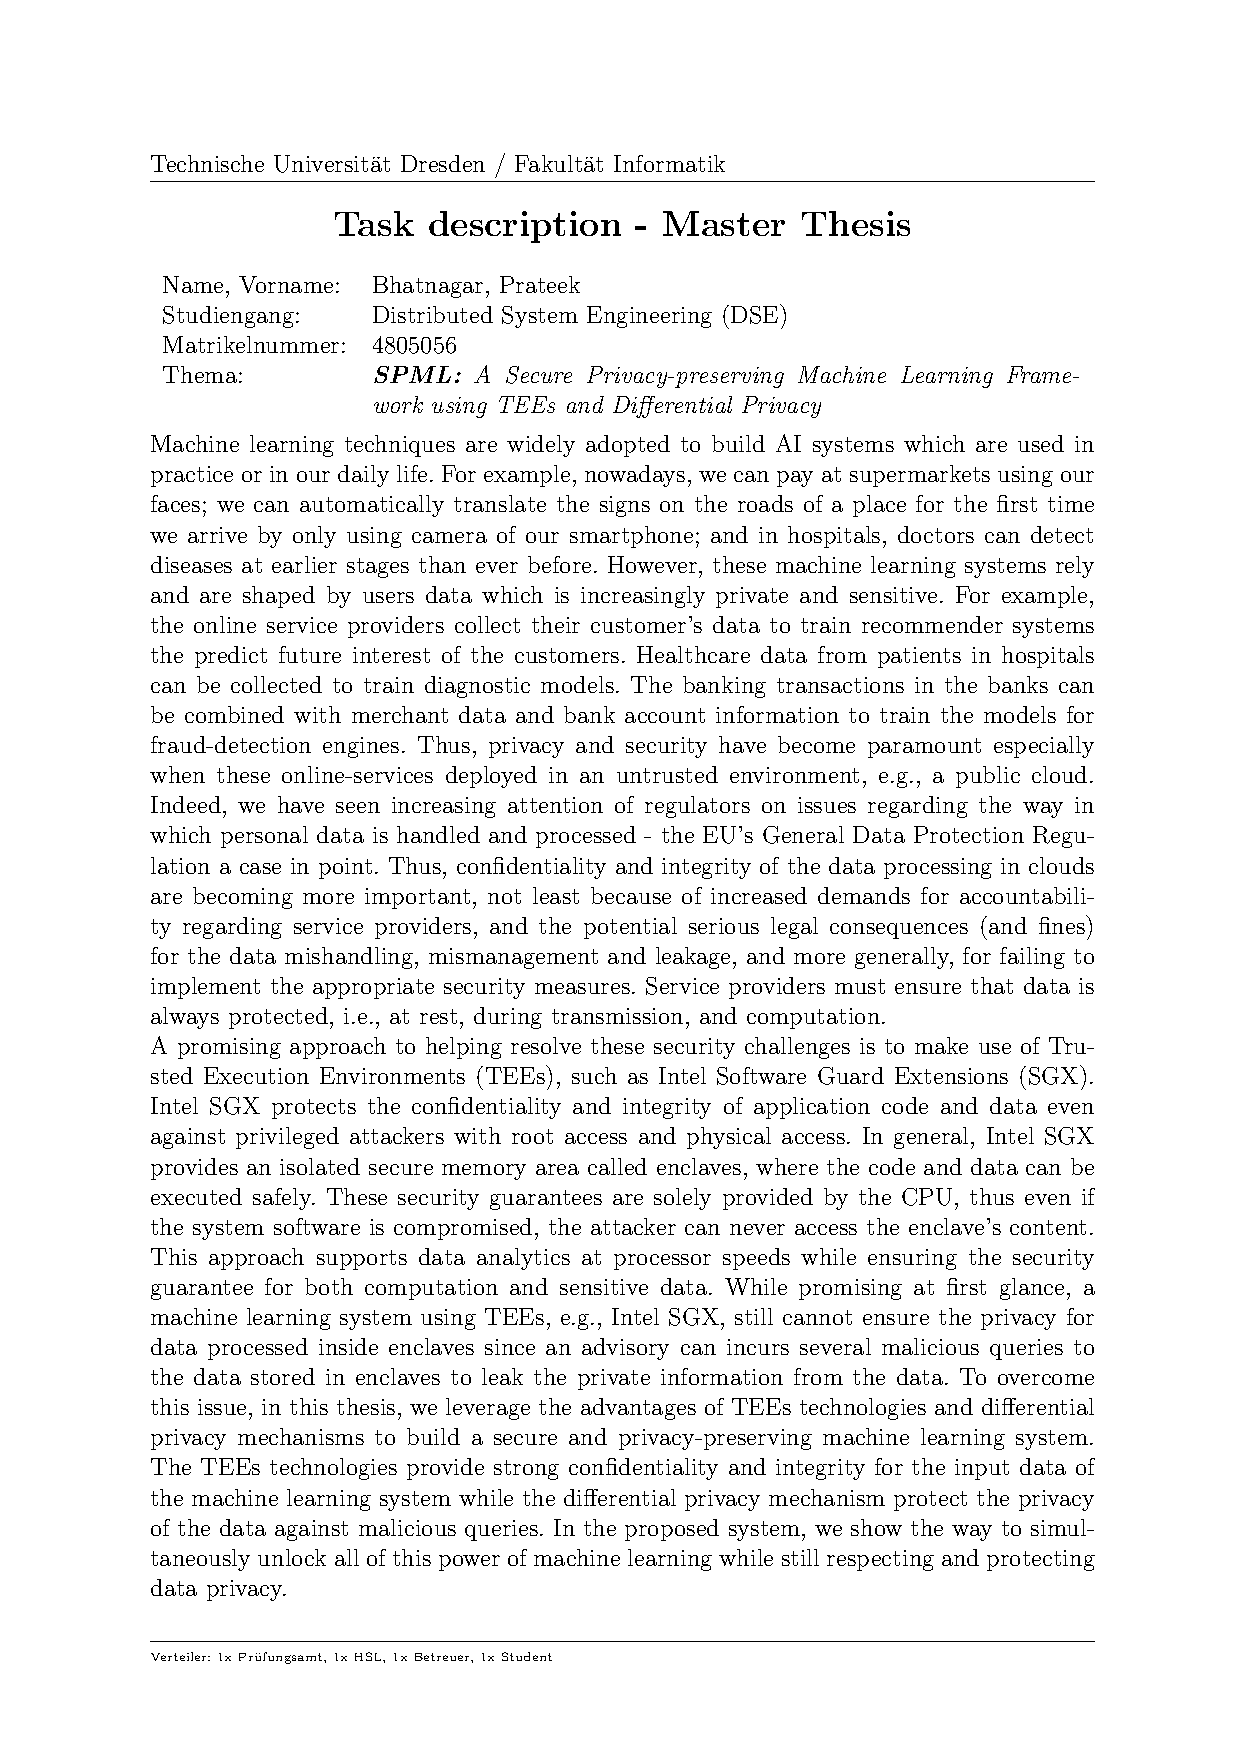
\includepdf[]{content/Td-1.pdf}
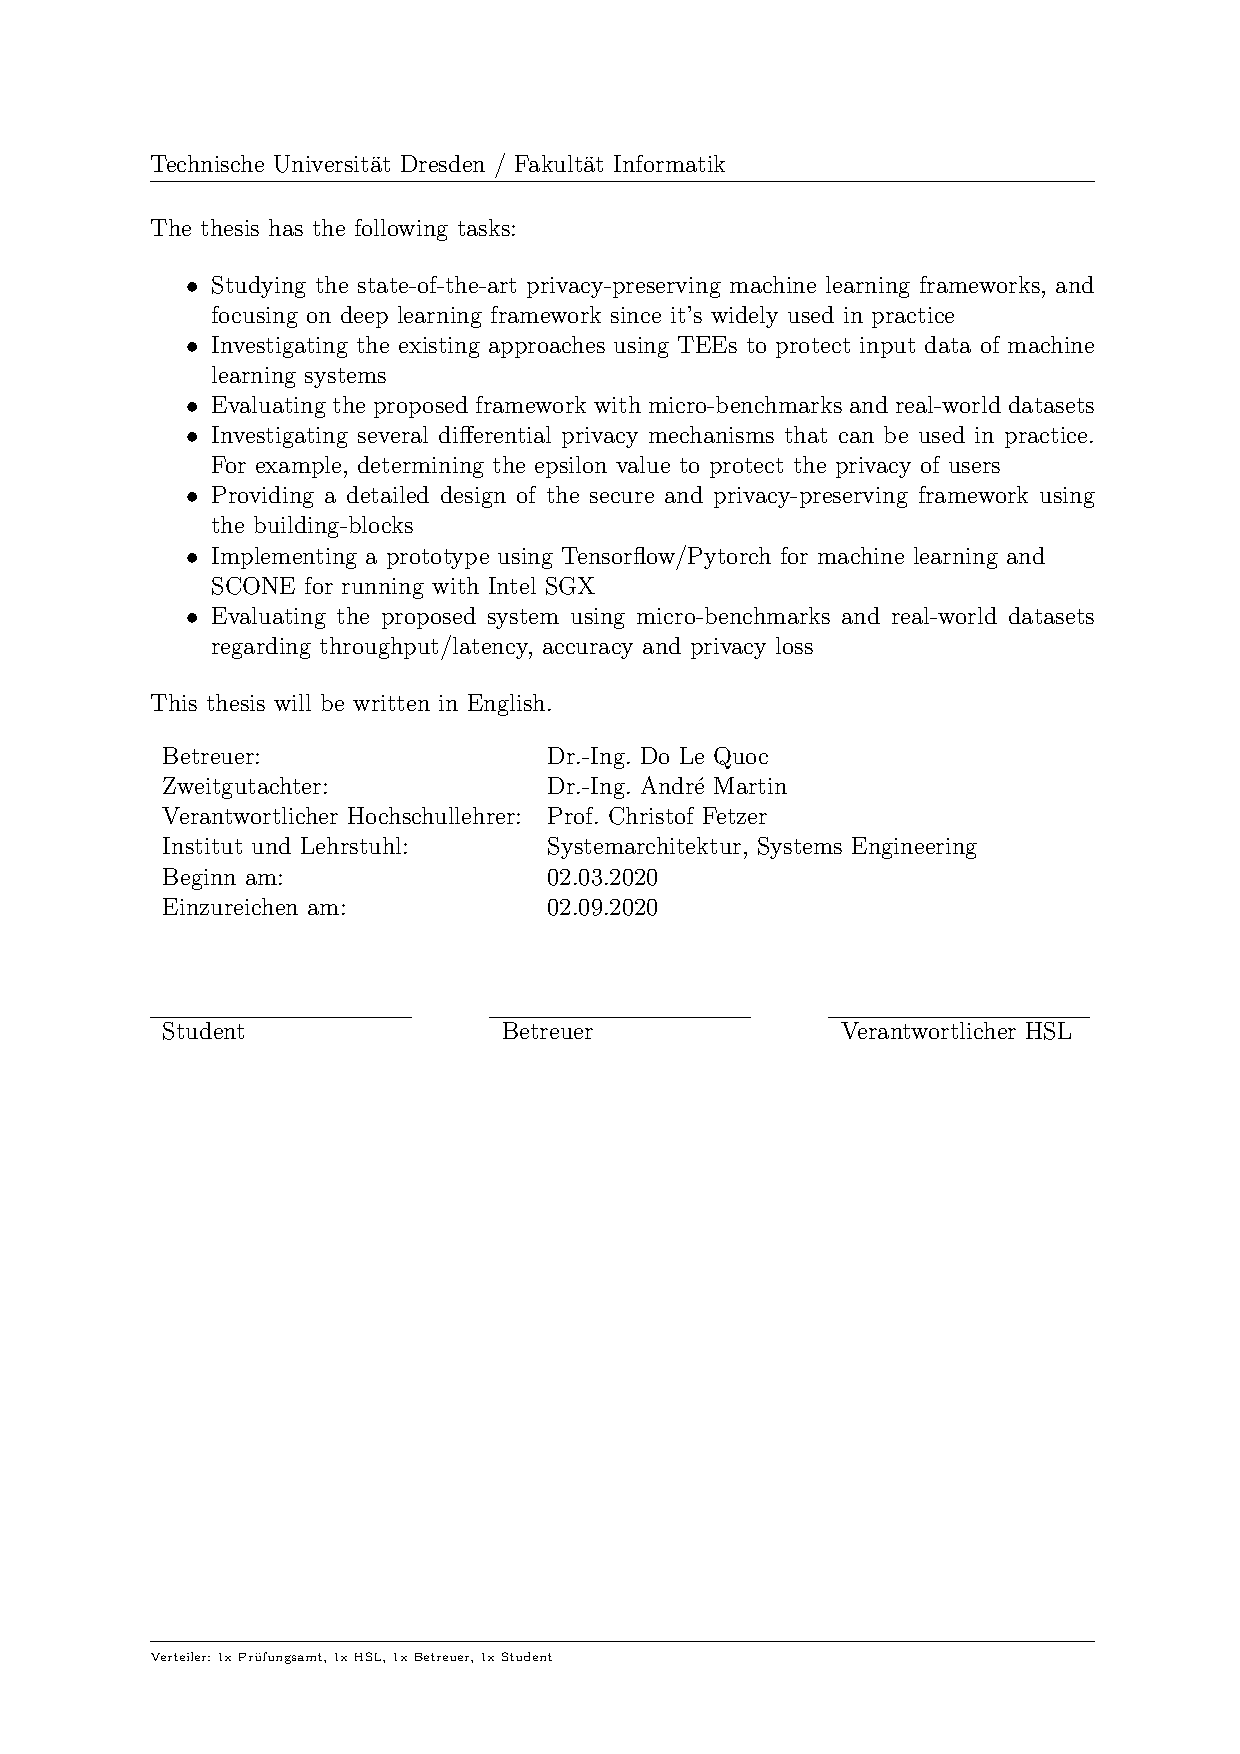
\includepdf[]{content/Td-2.pdf}
%\cleardoublepage

% -*- Mode: Latex -*-

\selectlanguage{american}
% \section*{\vfill{} \thispagestyle{empty} Declaration}
%\section*{}\thispagestyle{empty}
%\vspace{2.5cm}

\includegraphics[width=\textwidth]{content/Disclaimer.pdf}


%\cleardoublepage

% -*- Mode: Latex -*-

\selectlanguage{american}

\section*{}\thispagestyle{empty}
%\vspace{2.5cm}
\section*{Abstract}
\addcontentsline{toc}{chapter}{Abstract}
% \section*{\thispagestyle{empty}Abstract}
Machine learning techniques have been popular these days and are extensively used in many AI applications. These services are deployed in the public cloud for high performance, scalability, and availability purposes. However, security and privacy are major concerns for these systems when deployed in an untrusted public environment such as the public cloud. By security it means protecting the confidentiality and integrity of data and systems. One of the most emerging and promising approaches to protect the confidentiality and integrity of the data and system in an untrusted environment is to use the Trusted Execution Environment (TEEs) \cite{59}. 

The privacy means no private information about an individual should be leaked from the data. However, TEEs still cannot ensure the privacy of an individual. An adversary can still fire malicious queries on the trained model and private information can be leaked. Hence, some additional mechanisms and techniques are needed to preserve the privacy of an individual. One such popular and efficient technique to preserve privacy in a machine learning system is to use differential privacy \cite{3}.  It aims to learn desired information about a group while learning nothing about an individual in that group. 

We developed a system SPML that marriage privacy together with security (confidentiality and integrity). We have used TEEs to address the confidentiality and integrity concerns. Privacy is addressed using differential privacy. We evaluated SPML against MNIST \cite{12} and CIFAR \cite{13} dataset in the evaluation chapter ~\ref{sec:eval}. We learned that at stronger privacy bounds the accuracy of SPML decreases and while at weaker privacy bounds the accuracy is within an acceptable range. It is concluded that there is always a trade-off we have to make between accuracy and privacy level. Secondly, training the model takes a longer time as compare to inference, hence inference can be used in practice. However, we have discussed some advanced features also which can help to reduce training time taken to train the model.

Our system SPML, not only makes any native existing machine/deep learning system privacy-preserving but it also provides confidentiality and integrity. SPML is not only easy to use for new developments but any existing native machine learning system can use our system SPML framework and with minimum code changes privacy and security properties can be added in these native machine learning systems.
\clearpage
% -*- Mode: Latex -*-

\selectlanguage{american}

\section*{}\thispagestyle{empty}
%\vspace{2.5cm}
\section*{Acknowledgements}
\addcontentsline{toc}{chapter}{Acknowledgements}
I would like to thank and express my sincere gratitude towards \textbf{Prof. Dr. Christof Fetzer} for giving me this opportunity to work on this super exciting and futuristic thesis at the Chair of Systems Engineering.

It was not an easy phase to work remotely on the thesis in the COVID-19 situation. However, my adviser \textbf{Dr.-Ing. Do Le Quoc} keeps me motivated to do things perfectly by providing constructive and honest feedback always. I want to thank him for putting such extra efforts for me.

I also want to thank my \textbf{parents}, \textbf{sister} and \textbf{friends} who always supported and gave me early feedback. A very special thanks to my friends who always supported me by staying around me and taking care of daily errands in the COVID-19 situation for me.


%\cleardoublepage


% NOTE: if you selected british or american above, change that here too
\selectlanguage{american}

\tableofcontents
%\cleardoublepage

\printglossary[type=\acronymtype,style=long]
%\cleardoublepage

\listoffigures
%\cleardoublepage

%\lstlistoflistings
%\cleardoublepage

\listoftables
%\cleardoublepage

\pagenumbering{arabic}

\chapter{Introduction}
\label{sec:intro}
The machine learning \cite{65} aims to construct systems or applications that learn and improve with experience. Over the years, many machine learning systems have been developed which range from detecting fraud-detection \cite{56} for banking transactions, to facial recognition that can be used to pay at the supermarkets, to autonomous driving systems. In the medical field, diseases can be detected at a much early stage nowadays by training diagnostic models using patient's data in a hospital. The e-commerce players use a recommender system \cite{55} to suggest new products to the user based on their previous or historical data. However, machine learning is highly dependent upon private and sensitive user data. With all this data around for a long time, many attackers or adversaries try to steal this data, and hence this level of sensitive data needs protection from all such attacks in an un-trusted environment, for example, a public cloud. EU's General Data Protection Regulation (GDPR) \cite{57} is implementing stricter norms to define how user data should be handled and processed. As a consequence, the confidentiality and integrity of this data have become of paramount interest in an untrusted environment. Service providers need to adhere to both accountability and legal consequences for data mishandling, mismanagement, and leakage. Data must be protected not only during transmission and computation, but also when it is at rest.


In this thesis, we aim to build a machine learning framework that not only provides confidentiality and integrity to the data, code, model, and computation, but also provide privacy to the application. Confidentiality here means that the data, code, or model used for computation should be revealed only to the intended audience. Integrity means any kind of modification to any of these should be possible to detect. Confidentiality is usually addressed with the help of encryption/decryption. Encryption transforms the plain text to conceal it while decryption transforms the encrypted text into plain text. These techniques are achieved with the help of a single key or public-private key-pair. The integrity part is handled using message authentication which is the signing of data with cryptographic hash/signature \cite{58}. The details about confidentiality and integrity techniques are out of the scope of this thesis however can be studied in detail at \cite{58}.

To ensure the confidentiality and integrity of the cloud-native applications Trusted Execution Environments (TEEs) \cite{59} has emerged as one of the most promising technology. TEEs are hardware-assisted solutions that securely isolate the memory area through enclaves. Within these enclaves the data, code, model are executed safely and securely. Even if an adversary or attacker can compromise system software with root privileges, it is nearly impossible for an attacker to access the enclave's content (where the sensitive and private data/code is kept). There are many TEEs available in the market such as AMD Secure Processor \cite{19}, ARM Trust zone \cite{20}, Intel SGX \cite{9}, IBM secure execution \cite{21} etc. 

However, TEEs SDKs are complex, there are a lot of code changes required in the existing system for using TEEs SDK. To overcome this problem, we will be using the SCONE \cite{22} which provides a platform to run any existing application over TEEs without any code changes. Together with this combination, confidentiality and integrity can be added to any existing native application. For this thesis implementation, we choose Intel SGX as our TEEs because SCONE is currently developed using Intel SGX and both of these are well tested for performance and compatibility together.

TEEs look very promising to provide confidentiality and integrity guarantees however TEEs still cannot ensure privacy because an adversary can still hit the enclaves with the malicious query to the data which is inside the enclave and private information can be leaked by such queries. The privacy of the data means no private information about an individual should be leaked from this data. The adversary can query the dataset to gain some group information and with some prior knowledge about the subject, it can infer information with the help of multiple summary statistics queries such as count, sum, or average \cite{72}. Applying such attacks to the machine learning system can further lead to leakage of data, model, or model parameters. All such attacks on the machine learning system are discussed in detail in section ~\ref{sec:attackOnML}.


There are many techniques to achieve privacy goals such as approximation of activation functions with low degree polynomials \cite{60}, CryptoNets \cite{61},  SecureML \cite{62}. In our system SPML, we will be using a state-of-the-art privacy-preserving technique known as differential privacy proposed by Cynthia Dwork from Microsoft Research\cite{3}. Differential privacy \cite{3} states that no information about an individual should be learned from the dataset, while useful information about a population can be learned. For example, it can be learned from a medical database that smoking causes cancer, but it shouldn't be learned who all smoke. Hence, this notion about individual privacy can be protected using differential privacy. 

Recently there is a paper by Google \cite{4} to implement differential privacy, however, confidentiality and integrity guarantee is not ensured by this. We marriage privacy with confidentiality and integrity together in this thesis. To implement our system, we will be using TensorFlow \cite{46} framework by Google, Intel SGX \cite{9} as TEEs, and privacy paper by Google \cite{4}. We also explored a randomized response mechanism which is our contribution and work. In the evaluation chapter, it is shown that our system SPML provides confidentiality, integrity, and privacy guarantees however SPML makes training 25x and inference 6x slower as compared to the native system. We can say this is the cost of enabling security and privacy property for any existing machine learning system. The main advantage of using SPML is that with minimum code changes we can build any existing native machine learning or a deep learning system, a secure privacy-preserving system. SPML can be used with any cloud-native application and we can benefit from any cloud environment features like auto-scaling. The efforts required to change any existing machine learning application are very less and hence can save a lot of time required to add privacy, confidentiality, and integrity guarantee to the native machine learning system.

The thesis is organized in the form of different chapters. In the next chapter, some already existing work on these similar lines is discussed. After that background information about various technologies used in our system SPML is discussed in chapter 3. Chapter 4 talks about the design goals and detailed design of our system. Chapter 5, we have discussed the implementation details of our system. Chapter 6, evaluates our system for its performance and accuracy. Chapter 7 we have highlighted enhancement and future work required for making our system more usable. At the end of Chapter 8, we have concluded our work.

\chapter{Related Work}
\label{sec:related_work}
Our system SPML consists of a machine learning module, a privacy module, and a security component. The machine learning aims to provide the learning ability to the systems by training a model on the input data. These trained models can be used to predict or classify real-world data. The input data used for training these models contain sensitive and private information about an individual. Hence, confidentiality, and the integrity of an application, and the privacy of the individual whose data is involved in the dataset must be protected. We will be using differential privacy techniques \cite{3} in this thesis to address privacy concerns and Trusted Execution Environment to protect the confidentiality and integrity of an application. Differential privacy technique works by adding random noise on the input dataset. There are already many techniques proposed in the past about how to apply differential privacy on machine learning algorithms. We will discuss a few of these techniques first using a survey paper on differential privacy and machine learning and then later some start-of-the-art techniques as proposed by Google.


\section{Differential privacy and machine learning: a survey and review}
\label{sec:rwDPsurvery}
In this survey paper \cite{6}, a basic notion is discussed how differential privacy and machine learning can go hand in hand. At a high level, combining machine learning with privacy always requires a trade-off between privacy and accuracy level. This is because if too much noise is added to the input data, then data will become unusable as accuracy will reduce drastically. Hence, it requires some calibrated balance between accuracy and privacy. For example, if medical research is considered, it demands access to patient's records and at the same time, their privacy must be preserved. The challenge here is how to share generic information of patients without compromising their privacy. This problem is solved using differential privacy techniques \cite{3} which were proposed by Microsoft researcher Cynthia Dwork.

One could argue that if names and personal IDs are removed from the dataset/database, then data will be anonymous, as an adversary cannot learn anything about a person. However, if the adversary has some other related knowledge also known as auxiliary information about the user then such details can be used to conclude information that an adversary is looking for. For example, if a healthcare database from a hospital and voter registration information are combined, one may identify an intended person from the records by combining these two databases. Differential privacy introduces random noise in the publicly available data so that changes cannot be detected even if one row in the database is changed. Since the output is not dependent much on inputs, the adversary cannot get sensitive or any kind of information for any individual.

There are several groups of differentially private machine learning algorithms based on the approaches they use to preserve privacy. The first category is learning a model based on the raw data, then later applying the Laplace mechanism as proposed in \cite{26} \cite{27} \cite{28} \cite{29} \cite{30} or exponential mechanism using one of the techniques discussed in \cite{31} \cite{32} to generate privacy-preserving algorithms. In the second approach instead of first training the model on raw data, Laplace and exponential mechanisms are enforced on the output parameters after every iteration or step such as discussed in \cite{33} \cite{34} \cite{35} \cite{36} \cite{37} \cite{38} \cite{39}. The third category also known as objective perturbation is discussed in \cite{40} \cite{41} \cite{42} \cite{43}. In this type, the target function is made noisy by adding some noise to it and a minimum or maximum of this noisy function is used as an output model. The fourth category is based on the framework of sampling and aggregation as stated in \cite{44} \cite{45}. They work by splitting the input into several subsets, then the model is estimated by combining the results of all these subsets, and noise is added in the step of aggregation. 

However, all these papers and mechanisms don't define a general framework that can be used to train any kind of model. For example, if we are interested in applying the first approach, then it can be applied to train models using a few of the machine learning algorithms. The paper discussed in \cite{26} can only train models using naive Bayes classification. We cannot apply the same technique to train a model using a decision tree or logistic regression. Secondly, most of the approaches require us to either preprocess inputs or change the training algorithms which means adding a further overhead of changing existing code, which requires more effort. Most of this work is based on a convex model that has fewer parameters as compared to complex networks. Training complex networks that contain a large number of parameters such as deep learning models results in large privacy loss using these approaches as stated in \cite{4}. Hence, we need a framework that is generalized and can be used for any already deployed machine learning and deep learning systems with minimum code changes and efforts. Google has been actively contributing to this area and came up with paper for RAPPOR \cite{5} in 2014 which tries to explain how a randomized response mechanism can be applied in general to achieve differential privacy. We studied this paper to see if this paper addresses some of these shortcomings.

\section{RAPPOR-Randomized Aggregatable Privacy-Preserving Ordinal Response}
\label{sec:rwRappor}
RAPPOR paper \cite{5} talks about the start of the art method of achieving differential privacy using a randomized response. Most of the chrome users face an issue wherein an attacker wants to change the default home page on the browser but to find more about this type of attack, one needs to know what kind of homepages are used by the users which means invading the privacy of the user. The approach is to find an algorithm that aims to find a popular percentage of homepages or search engines like yahoo, bing, google, etc that are being used. RAPPOR finds the distribution of search engines without compromising the security of a particular user. It implements privacy to learn user statistics by imposing privacy guarantees for each user, and user data is not maintained in a database, hence there is no third party involved to put the trust into.

RAPPOR is built using the idea of randomized response \cite{14} proposed by Warner in the 1960s to collect survey results from people, wherein the confidentiality of the people participating in this survey is retained. This means after collecting data from many people, information can be learned about the population but nothing can be learned about the individuals participating in the survey. The approach here is that the URLs are converted to bloom filters and a subset is chosen from a big bit vector, and noise is added there. RAPPOR is executed on the client locally and the report is sent to the server. 


The algorithm is based on the client's value v and some parameters such as f, h, k, p, and q. First, the client value v is hashed into the bloom filter say B having size k with the help of h hash functions. Then a permanent randomized response B' is created for each value v and bits in the B with the help of probability f. The parameter f is a tunable parameter to control the longitudinal privacy guarantee level. B' is memoized and reused in all subsequent reports for this value v. The next step is to generate instantaneous randomized response S. S is obtained by modifying B' with the help of probabilities p and q. Then S is sent to the server. In the paper, it is also shown how differential privacy levels can be controlled with the help of these parameters.


 This paper shows the state-of-the-art way to use a randomized response mechanism to achieve differential privacy guarantees. It works well for heavy-hitter collection, but what about the scenarios in which the client answer changes with time even for the same query as point out in \cite{18}. The RAPPOR target a particular type of problem however, applying this in all variety of machine learning problems such as image or object classification, which are based on deep learning techniques, still require some more effort and work.
 
 Secondly, a user can log in through different devices like phone, PC, tablet, etc which may lead to another problem of information leakage if all these data is collected for a single event. Also, the number of the cohort (subset chosen from big vector) must be changed as it may help to track the clients and can reduce privacy. RAPPOR protects the privacy of the training dataset but what about protecting the model’s parameters. An adversary can use the trained model to attack the machine learning system using model inversion attack \cite{17} or membership inference attack \cite{16}. Hence, we need some other mechanism that protects the training dataset and the trained model’s parameters.

Google came up with paper for Deep Learning with differential privacy \cite{4} in 2016 which tries to generalize the application of differential privacy in any kind of machine learning framework including deep learning. It not only protects the training dataset but the model’s parameters also.
 
\section{Deep Learning with differential privacy}
\label{sec:rwDL}
In this paper \cite{4}, advanced privacy-preserving mechanisms are combined with state-of-the-art machine learning methods to train neural networks. Broadly in machine learning, there is a feedback loop wherein customers are motivated by the high utility of an application or platform and hence they are ready to share more and more private and sensitive data with the devices and computing platforms. All these devices and platforms become more powerful with the data shared with them. As per the standard pipeline for machine learning, training data is fed to the trained model and the inference engine uses these models to make inferences. 

Authors argued that machine learning systems already have techniques like regularization which can protect the training data. On the other hand, deep learning networks have complex internal representations and these representations might leak some of the information about training data as demonstrated in model inversion attack \cite{17} or membership inference attack \cite{16}. Hence authors have implemented and evaluated the algorithm with deep learning methods. 

This algorithm will not only protect the training dataset but also the model’s parameters. This algorithm has been implemented in TensorFlow \cite{46} released by Google in 2015 and aims to build a differentially private stochastic gradient descent algorithm (SGD). In the algorithm, the loss function is minimized at each iteration. It consists of computing gradient at each step for a random sample from the dataset, clipping the l2 norm of these gradients, computing the average, and then adding random noise to preserve privacy. 

To compute the privacy loss of this differentially private SGD, a privacy accountant \cite{49} procedure based on the composability property of differential privacy is used. Privacy cost is calculated on the training data on each access and is accumulated with the progression of training. Gradients are calculated for each iteration of training and this accountant is responsible for accumulating the cost for all of these iterations.

Hence, this work gives us the generalized framework to apply differential privacy not only on machine learning techniques but also on deep learning network techniques. Therefore, using this algorithm privacy of the data can be preserved even in complex networks. 

However, this paper doesn't talk about how to preserve the confidentiality and integrity of the data, model, code, and inference results in an untrusted environment. We can use this work for solving the privacy problem but security concerns cannot be addressed using the techniques discussed in this paper. This is where Trusted Execution Environments (TEEs) comes to the rescue, to provide the confidentiality and integrity to the applications.

\section{Trusted Execution Environment}
A trusted execution environment (TEE) \cite{59} aims to provide confidentiality and integrity to the data and code. It achieves this goal by executing code and data isolated from the other processes. An isolated memory region called enclave is defined where the code and data are executed. This isolation happens by utilizing hardware as well as software approaches. The chip contains private keys generated by the manufacturer, which protects the TEE content by any untrusted parts (i.e OS or hypervisor process or even root user) of the platform. 

One may argue that there are many existing software techniques for preserving the confidentiality and integrity of the data and code such as homomorphic encryption. With homomorphic encryption, encrypted data and model can be processed without decrypting them during training for machine learning or deep learning task, however, it incurs a high computation cost \cite{50} \cite{51}. On the other hand, TEEs don't incur such a high computation cost and its performance can be compared with the native runs of the untrusted environment such as public cloud for deep learning network \cite{52} \cite{53}. Hence, TEEs are a better choice in our case instead of using any other software approach/es.

The only problem with TEEs is that we need to change the native code of the application and add hardware instructions in the application to utilize benefits on TEEs. This requires an understanding of an additional set of hardware instructions and code modification which is an overhead for the developers. We overcome this overhead by using SCONE (Secure CONtainer Environment) \cite{22}. The SCONE is a confidential computing platform that facilitates execution in always encrypted form. The additional overhead of input/output encryption, application execution in isolated (encrypted) memory is simplified by SCONE. The SCONE is discussed in detail in the next section.

%\cleardoublepage

\chapter{Background}
\label{sec:background}
In this chapter, the main focus is on the basics concepts used in the thesis. We will start with the basic process of machine learning, what are the types of attacks exist for it. Then some concepts about TEEs and differential privacy are explained which we will use to develop our system SPML.
\section{Machine learning}
Machine learning \cite{65} aims to build a system that learns with experience. It is a mix of statistics and computer science. Machine learning is widely used in every field of technology, science, and commerce such as education, health care, finance policing, marketing, etc. The machine learning comes under the study of artificial intelligence. Many Artificial intelligence (AI) based systems such as speech recognition, computer vision, robot control, natural language processing are using machine learning for their software development. Machine learning consists of data or database as an input, a training model, and predictions/classification as output. It consists of two phases training phase and the inference phase. The training phase trains the model with the help of input data and the inference phase is the one in which this trained model is used to predict/classify the real-world problem. These phases are discussed in brief as follows.

\subsection{Training Phase}
In this phase, the model is trained to predict output or classify something such as an image. It consists of reading the input, prepossessing the input (making it suitable to feed into the model), defining a model, choosing a loss function, and an optimizer. The model has some parameters which help to deduce output based on the input. For example, to predict the average salary of an individual, the input can be education qualification, years of working experience, occupation, etc, and output will be salary. 

\begin{figure}
    \centering
    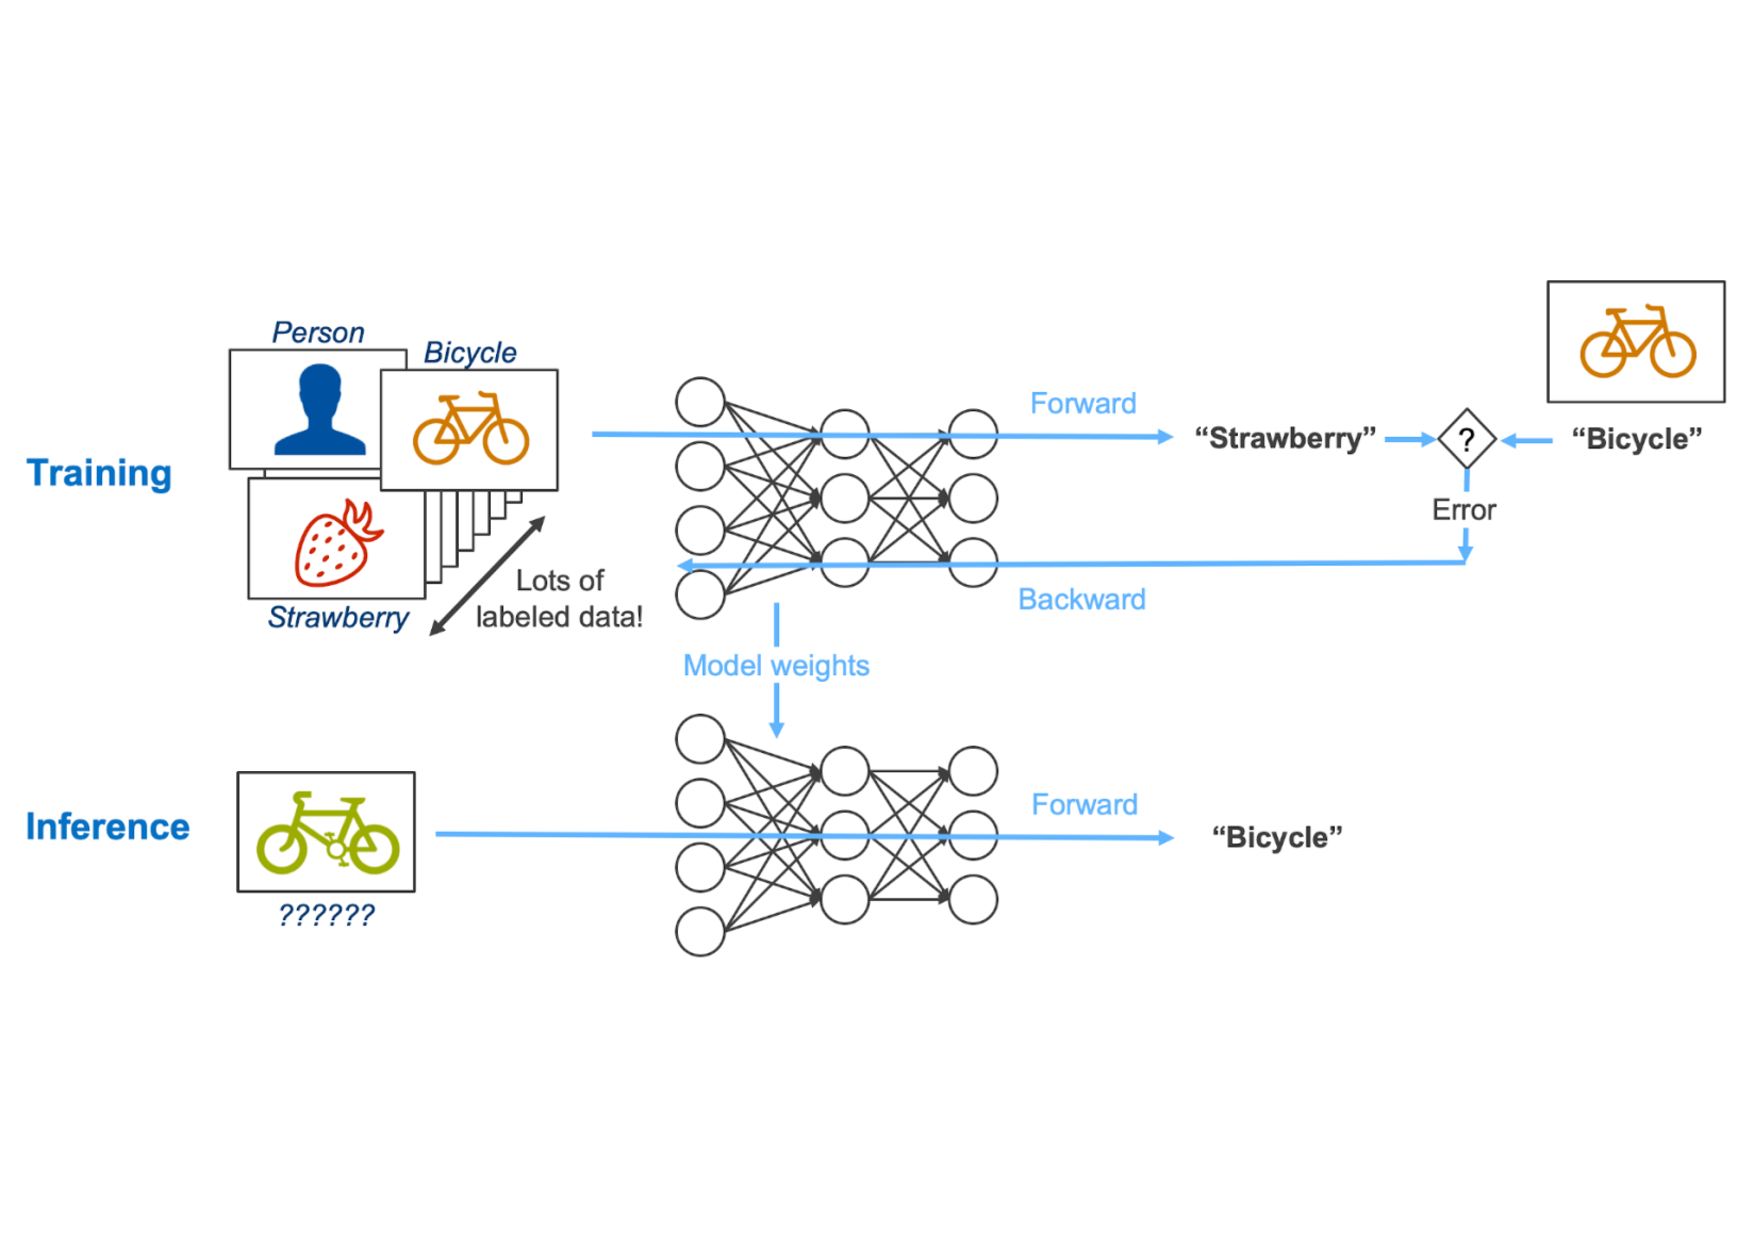
\includegraphics[width=10cm, height=10cm]{images/Background/config.pdf}
    \vspace{-6em}
    \caption{Training vs Inference Phase \cite{82}}
    \label{fig:backgroundTI}
\end{figure}

In general, the training phase tries to find the nth (column) point using (n-1) points (columns). The input data set is made up of some n points (columns). The main goal of training is to find the optimal settings to achieve the maximum accuracy so that the nth point can be predicted/classified correctly using n-1 points. The goal of the loss function is to find how well the current model is performing on predicting/classifying the target (training) data. For example, if there is too much deviation from the expected value, then the loss function will be very high. On the other hand, the optimizer function helps to minimize this loss. Hence, the training phase includes the main computation where the loss function calculates the loss or deviation from the expected values, and the optimizer function tells how to minimize the loss by adjusting various model's parameters. The adjustment of the model's parameters is a lengthy process and takes multiple iterations to find the optimal values. The accuracy of the model is calculated using these model's parameters and is an important parameter to decide when to stop the training.

For example, in Figure ~\ref{fig:backgroundTI} the neural network is trained to classify images into three categories which can be a strawberry, a bicycle, and a person. The training data has a lot of images and these images are labeled as strawberry, bicycle, and person. Each of the images will be passed through different layers of network and the network is trying to classify these images into a person, bicycle, or strawberry. It might be possible that during the training a bicycle image is classified as strawberry which is incorrect. To handle this, the error will be propagated back to the network, and model weights are corrected so that the next time model classifies the image into the correct category. This process continues where images are fed to the network and weights will be updated again and again to correct such errors. The training process is continued until the model is achieving the desired accuracy level. Once the model is trained with sufficient accuracy it can be used to inference, which forms the next phase of any machine learning system.
 

\subsection{Inference Phase}
This phase act on the trained model obtained from the training phase to predict/classify unseen data. The trained model is of small size and hence can be easily deployed in any device or computing platform such as cloud or smartphones, etc. It can be used to inference real-world data. With a well-trained model, one should get almost the same accuracy with real-world data as got during the training phase. Its a compress, simple, and optimized version of the training phase. For example, in Figure ~\ref{fig:backgroundTI}, when the image is fed into the trained model, the model classifies correctly it as a bicycle. The model uses model weights obtained from the training phase to make an inference.

In terms of performance, the inference phase is much faster than the training phase because, in the inference phase, we don't need to adjust any model's parameters which is the most time-consuming part in the whole machine learning process. A well-trained model will be able to do right predictions as much as possible for real-world data. Despite all the advantages that machine learning offers it also suffers from a few challenges such as the curse of dimensionality.

\subsection{Challenge of machine learning}
Machine learning cannot solve many important problems of AI such as speech or object recognition \cite{65}. Machine learning problems don't perform or fit well when the data has a lot of dimensions. This problem of high dimension is called a curse of dimensionality. If there are more dimensions there will be more variables and machine learning algorithms don't perform well in such scenarios. Machine learning algorithms have high computation costs and cannot learn complex functions in such high dimensional spaces. Hence machine learning cannot generalize all the problems in AI. To address such issues and apply machine learning in general, deep learning technique is widely used to solve the aforementioned problems.

\subsection{Deep learning}
Deep learning is a specific type of machine learning \cite{65}. It aims to solve the problem in representation learning such as speech or object recognition. It tries to present these representations into more simple representations so that complex concepts can be built out of simpler ones. To get an idea about this concept, let us understand the basic model in deep learning knows as multilayer perception (MLP). It maps input values to output values. It consists of a much simpler function and together they compose further complex functions. 

For example, if we take image classification then, the computer cannot understand the sensor input as an image. However, images can be represented as a collection of pixels. Deep learning breaks this complex problem into many nested mappings. All these nested mappings can be described by a different layer in the model. The first layer generally known as the input layer holds observable values. Thereafter, other features from the image are extracted by hidden layers after the input layer. With the help of pixels, input layers can detect edges of the images. Once edges are detected next hidden layer can detect for corners and contours and then the next hidden layer can detect specific objects. Once the object is detected, it is easy to identify if that object is a part of the image or not. Hence the complex problem is solved by dividing the problem into multiple stages or layers. This is how deep learning solves any kind of problem which can be speech, object recognition, or simple prediction problem.

Machine learning and deep learning are related to each other. Briefly, we can say machine learning is one approach to build AI systems and deep learning is a kind of machine learning that provides flexibility in representing real-world problems. However, machine learning/deep learning is not free from attacks, an adversary can try to steal the data from the training set or poison the data to sabotage the training process. We need to protect our data, model, and computation with all such attacks. To protect our machine learning or deep learning system against such attacks, first, we need to understand how various attacks can happen over these systems.

\subsection{Attacks on machine learning}
\label{sec:attackOnML}
In this subsection, our focus will be on privacy attacks on the machine learning system. In general, to attack a database and to gain private information inference attacks \cite{71} are commonly used. In this attack, data is analyzed to gain knowledge of an individual or subject. For example, the adversary can query the database to gain some group information and with some prior knowledge about the subject, it can infer information with the help of multiple summary statistics queries such as COUNT, SUM, or AVERAGE \cite{72}. Machine learning is purely based on the training model on some datasets/database, hence machine learning models can be attacked using inference attack easily. Some popular inference attacks known for machine learning are as follows.
\subsubsection{Model inversion attack}
In model inversion attack, as stated in \cite{17}, if an adversary has access to a trained model and some auxiliary information about an individual then it can make predictions about an individual's genetic markers. This particular attack is discussed via an example from the pharmacogenetics field in the paper, but it can be generalized for any scenario. It is assumed that only researchers have access to datasets and only the model learned from these datasets is made public. It is a black box type of attack, datasets are private and not accessible by an adversary. However, an adversary can exploit the correlation between unknown attributes, model output, and target information. This means an adversary has access to a trained model only and using this model it can easily deduce input attributes passed to the model.

It is a security and privacy risk to the applications based on such trained models. It is proved in the paper that, if an adversary knows the intended individual's background and dosage, then it can predict their genetic markers with good accuracy. This will compromise the privacy of an individual and we need to protect that. To prevent such attacks, the author used state-of-the-art differential privacy mechanisms to produce trained models and it was concluded that genomic privacy is protected for a small value of $\epsilon$. Hence, to some extent, such attacks can be prevented using differential privacy.

\subsubsection{Membership inference attack}
Membership inference attack, \cite{16} states that if access is given to a machine learning model, then is it possible to determine whether a record was used to train this model is present or absent in the training dataset. It is a black box type of attack where an adversary can only fire queries to get output for the given input. In this attack, machine learning is used against itself. 

Authors used a technique called shadow training which creates shadow models. To develop training datasets for these models, there are few methods discussed in the paper \cite{16} and can be referred for more details. These model's behavior is then imitated for the target model. The attack model is trained using these shadow models which converts this inference problem into a mere binary classification problem. Authors have suggested that to mitigate such types of attacks differentially private models can be used. The differentially private trained models are immune to membership inference attacks like in this case where only model output is known and no auxiliary information is known to the adversary.

\subsubsection{Model extraction attack}
Model extraction attack \cite{73} is also a black box attack. In this, an adversary tries to steal the model functionality without knowing any training data or model's parameter. An adversary sees the model as a black box hence can query it. It can learn predictions on some input features by querying the model. It is also assumed that the adversary doesn't know about training data distribution or model type (linear regression, decision tree or logistic regression, etc). This attack is successfully demonstrated for majority model types such as logistic regressions, SVMs, decision trees, and deep neural networks. If differential privacy prevents such type of attack or not is left for further discussion.

After going through all these inference attacks which try to learn either model parameters or if a particular record is in the training set or not, differential privacy proved to be a successful mechanism to avoid or prevent these types of attacks. Hence, we decided to use differential privacy in our thesis to address the privacy concern. To understand what exactly is differential privacy, how to apply differential privacy, why it can avoid such attacks, we studied differential privacy in detail as explained below.
\section{Differential privacy}
Differential privacy (DP) \cite{3} was proposed by Cynthia Dwork from Microsoft research. It aims to learn desired information about a group while learning nothing about an individual in that group. This means that if an adversary tries to query some information out of this group, most of the responses will be equal, irrespective of any individual is present or absent in the group. For example, if a database of patient records is maintained by some hospital to indicate if some patient has cancer or not, then this information should not be leaked. However, if the hospital wants to release some data like the total number of patients with what type of cancer for research purposes. Then differential privacy defines if some adversary can intrude information then it shouldn't be learned that some particular individual has cancer. The assumption here is that the hospital is a trusted source and the database cannot be hacked by an adversary and hospitals want to protect patient privacy. Formally differential privacy is defined as:
\begin{itemize}
    \item $\epsilon$-\text{differential privacy} for some mechanism M:
        \begin{equation}
            \forall S , Pr[M(x) \in S] \leq exp( \epsilon ) . Pr[M(x') \in S]
        \label{eq:epsDP}
        \end{equation}
    where x, x' are any two neighboring data-sets, S $\subseteq$ range(M) and, $\epsilon$ is a measure of how much privacy is being leaked or also known as privacy loss.
    \item ($\epsilon$,$\delta$)-\text{differential privacy} for some mechanism M:
    \begin{equation}
        \forall S , Pr[M(x) \in S] \leq exp( \epsilon ) . Pr[M(x') \in S] + \delta
    \label{eq:epsdeltaDP}
    \end{equation}
    where $\delta$ is a small probability of failing.
\end{itemize}

After formally giving introduction and definition of DP, lets us discuss a few important qualities or properties which make DP an ideal mechanism to achieve privacy. There are many properties discussed in privacy book \cite{80} but here we will discuss only three properties which are important from this thesis point of view, these are :
\begin{itemize}
    \item  \textit{Composability}: If two or more independent components of a mechanism are differentially private then their union (composition) will also be differentially private.
    \item  \textit{Group privacy}: If the dataset has inputs that are correlated to each other, then privacy guarantees will be degraded gracefully.
    \item  \textit{Robustness}: The privacy guarantees are not dependent upon any kind of auxiliary information that is known to the adversary.
\end{itemize}

These properties make differential privacy special and important in achieving privacy. The next question is how we can achieve DP in our algorithms, what are different techniques to achieve it. Before discussing the techniques to achieve DP, let us discuss the sensitivity of a function that is used by these DP techniques to make any algorithm differentially private. In simple words, the DP is trying to hide if a particular person is present in the dataset or not. The presence or absence of one person shouldn't change the output. This means DP is trying to measure how much one individual can affect the output. Mathematically, we can say if there are two neighboring data sets say D1, D2 and some function f over D1 and D2, then \textbf{sensitivity of function f} is defined as how much this function f can change if applied on the D1 and D2 \cite{2}, this means we are trying to hide this difference, so sensitivity can be defined as:
\begin{equation}
\Delta f = \max(D1,D2) \mid f(D1)-f(D2) \mid
\label{eq:epsSentivity}
\end{equation}
The equation ~\ref{eq:epsSentivity} tells till what extend noise is added so that privacy is preserved. For example, if some data can be obtained by counting the number of rows in a database then such a query or function will have a sensitivity of 1. If one individual is added or removed from the respective database then this count will differ maximum by 1. Now it is clear that we are trying to hide the change in the dataset that can happen by adding or removing an individual and this change is defined in terms of sensitivity of a function f. This means some kind of uncertainty should be introduced in the answer to hide this presence or absence of an individual. The uncertainty can be added in terms of randomized response or some noise that will hide the presence or absence of an individual. Two of the most popular ways to add uncertainty to differential privacy is using randomized response or noise.

\textbf{Randomized response}
Randomized response technique is proposed by Warner \cite{14}, which is based on a coin flip. According to this technique, randomness is added to the response by each person. If simple questions are asked which can be answered in yes/no, then instead of answering these questions directly, some plausible deniability is introduced in the answers. According to Warner to answer a question: (1) A coined is flipped two times (2) If its head, question is honestly answered (3) If its tail, then second coin flip comes into play and yes is answered for the head and no is answered for the tail. This provides plausible deniability because it cannot be traced if the answer is honestly answered or its due to the coin flip. The advantage of using this type of noise is that it is easy to implement but the major disadvantage is that, to add randomization each dataset must be studied and re-engineered/pre-processed to add random noise to it. In practice, this is not feasible sometimes and the randomization can change the overall training dataset also. Hence, we need to think about some other mechanism where with minimum efforts we can introduce the uncertainty without changing the overall dataset. So, we looked into another mechanism which is to add random noise.

\textbf{Noise Mechanism}
In the noise mechanism, some calibrated random noise is taken from some mathematical distribution and added to the input/output. Two popular distributions that can be used to add noise are Laplace or Gaussian distribution, hence the names Laplace or Gaussian noise. Each of the noise is added using their respective parameter and mathematical questions. To add Laplace noise scale factor b is needed as explained in equation ~\ref{eq:epsLaplace}, while Gaussian noise needs variance which is calculated using equation ~\ref{eq:epsGaussian}.
\begin{itemize}
    \item \textbf{Laplace noise}
Laplace noise is based on the mathematical Laplace distribution. Random values are chosen from the Laplace distribution with mean 0 and scale factor b as :
\begin{equation}
b= Lap(\frac{\Delta f} { \epsilon})
\label{eq:epsLaplace}
\end{equation}
  \item \textbf{Gaussian}
Gaussian noise is based on the mathematical Gaussian distribution. Random values are chosen from the Gaussian distribution with mean 0 and variance $\sigma^2$  as :
\begin{equation}
\sigma^2=\frac{2\log(1.25/\delta).(\Delta f)^2}{\epsilon^2}
\label{eq:epsGaussian}
\end{equation}
\end{itemize}

In the machine learning system, there are many points at which these noises can be added such as before the training the model or during the training in computation functions or at the output after the training. These equations ~\ref{eq:epsLaplace}, ~\ref{eq:epsGaussian} just tell us how much noise should be added. However, where and how to add such noises over the machine learning or deep learning is already discussed in section ~\ref{sec:rwDPsurvery} and ~\ref{sec:rwDL} respectively. With differential privacy we can address our privacy concern, and, to address our confidentiality and integrity concern we still need some other mechanisms or tools. One of the most popular and computationally inexpensive ways to address these concerns is with TEEs. TEEs is one of the most promising and emerging approaches to achieve confidentiality and integrity in any system.

\section{Trusted Execution Environment}
Trusted Execution Environment (TEEs) \cite{59} is a way of executing the code and keeping data isolated from other processes. These are the hardware-assisted solution to add confidentiality and integrity to the code, data, and runtime states (such as memory, CPU registers, and I/O). To achieve confidentiality we need encryption/decryption keys and for integrity some kind of signed hash as discussed in ~\ref{sec:intro}. CPU provides secret keys for encryption/decryption to protect confidentiality and integrity of memory. To prove and trust third parties TEEs provide remote attestation.  Many implementation for TEEs are available such as AMD Secure Processor \cite{19}, ARM Trust zone \cite{20}, Intel SGX \cite{9}, IBM secure execution \cite{21}. For this thesis implementation, Intel SGX is chosen as TEEs. 

\subsection{Intel SGX}
Intel SGX \cite{9} was launched in 2015 and since then there are a lot of improvements over it. It extends the instruction set of x86 architecture by providing 18 new instructions and 13 new data structures. These sets enable the creation of a private memory region called as enclaves. Reading and writing are strictly prohibited in enclaves by any process outside the enclave even though the process belongs to a higher privilege level. A special memory region called Enclave Page Cache (EPC) contains enclave code and data. A dedicated chip known as Memory Encryption Engine (MEE) encrypts enclave memory. Hence, any reads by the processes outside the enclave will see this encrypted data. MEE is also responsible for encrypting pages before swapping and moving them into DRAM and decrypting these pages when the enclave wants to fetch data from DRAM. This means that the enclave code can still access the outside enclave memory while non-enclave code cannot access the enclave code. This also makes the overall computation a little bit slow due to small EPC size and paging, but we are achieving confidentiality and integrity for a system/application.

However, there are few challenges to use Intel SGX. First, to use Intel SGX one needs to know about the new set of hardware instructions and incorporate these new instructions into the application. This means source code changes are needed in the native applications. Secondly, an additional code is required for attestation and key provisioning. Thirdly, Intel SGX supports only C/C++ languages and is prone to side-channel attacks \cite{74}, hence we need some other environment to overcome these shortcomings. These challenges are overcome by SCONE (Secure CONtainer Environment) \cite{22}. SCONE provides transparency so that no code changes are required in the native applications. It supports many languages such as C, C++, Go, Rust, Java, Python, R, etc. It enables any native application to run inside Intel SGX enclaves. It takes care of secret key and configuration management and can handle side-channel attacks. It makes it easier to use Intel SGX and any native application can be run inside Intel SGX with help of SCONE. In the next subsection, we will discuss SCONE in brief.

\subsection{SCONE}
SCONE is a (Secure CONtainer Environment) \cite{22} based on Intel SGX and docker to run Linux based applications. Scone provides minimal TCB (Trusted Computing Base) hence a smaller attack surface. It provides transparency towards docker which provides easy deployment of container images, and less overhead by having user-level threading and asynchronous system calls. Compilation and linking of the applications are done with the help of a modified C library known as SCONE libc. To provide security, the address space of the application is restricted only to the enclave memory and the system call interface is used for any kind of interaction with the untrusted memory. Hence outside threads can execute these system calls asynchronously. Very minimal changes are required in an application to run it with SCONE. SCONE provides an environment to run applications inside containers on a trusted execution environment. Its main goal is to protect data always by encrypting it, whether data is resting, transmitting, or is in the main memory. Existing applications need not be modified to integrate with SCONE. SCONE supports all of the modern languages such as Python, Java, Go, C, and C++, etc and support is always evolving. Since source code is not modified so any native application can easily run on any TEEs. Hence, we decided to use SCONE in our system SPML so that our system can take all additional advantages that SCONE provides like containerization, generalization, ease of deployment, etc.

%\cleardoublepage


\chapter{Design}
\label{sec:design}
In this chapter, we will discuss the design of our system SPML. Our system SPML aims to protect the confidentiality, integrity, and privacy of the machine learning data and model so that native users don't have to change much of their existing system and yet can achieve stronger privacy and security guarantees. The system consists of two main parts, privacy which is fulfilled using differential privacy, and security which is fulfilled using Trusted Execution Environments (TEEs) for example Intel SGX, ARM TrustZone, etc. In this chapter, the detailed design of the proposed system SPML is described and how each component in the system is achieving our design goals. 
\section{Design Overview}
This section consists of design goals for our system SPML, threat models we are considering, and high-level design for it.
\subsection{Design goal}
All or most of the machine learning models are trained using private and sensitive user data. When such models are used in untrusted environments such as public cloud then privacy, as well as security is always the concern. The goal of any new system is to enable compatibility and usability with early versions so that the existing system can easily be upgraded and adapt to the new features. Keeping all such things under consideration SPML will be designed with the following design goals:
\begin{itemize}
  \item \textbf{Security}: The security means confidentiality and integrity of the data should be protected. To enable security property in SPML, Trusted Execution Environment (TEEs) are used. TEEs protects the application code, model and its parameters, and data inside an enclave and this isolation helps us to achieve our confidentiality and integrity goals.
  \vspace{-0.3cm}\item \textbf{Privacy}: An adversary can still fire many malicious queries on the dataset or trained model to retrieve information of an individual and can breach their privacy. SPML implements differential privacy techniques to preserve privacy.
  \vspace{-0.3cm}\item \textbf{Transparency}: System should be easy to access and use with minimum or no code changes hence APIs should be exposed for the usage of the system so that existing system or code can be upgraded or new features can be integrated easily. SPML uses the SCONE runtime environment which hides the complexity of using TEEs by providing a container-based platform to run any native application with Intel SGX. Additionally, SPML provides easy APIs and any existing system can make use of these APIs with very little code change.
  \vspace{-0.3cm}\item \textbf{Scalability}: It must be easy to scale up the resources of the system. This is one main feature of cloud these days wherein resources can be expanded or contracted easily depending upon the demand from the end-users. SPML being a containerized application support this functionality by default.
  \vspace{-0.3cm}\item \textbf{Performance}: Performance should be the same as the native performance with as little overhead as possible. SPML uses the most promising approach TEEs and start-of-the-art technique differential privacy to achieve security and privacy goals respectively. These approaches or techniques are currently the most optimized one in terms of performance and evolving continuously. Hence, any improvement in these areas will also help our system SPML to further improve its existing performance in the future also.
  \vspace{-0.3cm}\item \textbf{Accuracy}: Accuracy should not change much by enabling security and privacy property. SPML is tested against the hello world dataset of machine learning, MNIST \cite{12}, and CIFAR10 \cite{13} to ensure this.
\end{itemize} 
\subsection{Threat Model}
The goal here is to protect against an attacker in an untrusted environment infrastructure such as public clouds. In the cloud, most of the resources are offered via virtualization either in the form of VMs or containers. If an attacker can intrude in the system it can get hold of all the system resources such as OS, hypervisor, and can attack the system by doing memory dumps. In such a scenario application (code, data, model, and computations) confidentiality, integrity, freshness, and privacy must be preserved. Users can be trusted most of the times but sometimes an adversary might attack the system through inversion attacks i.e black-box queries which might leak data or model. Three types of attacks that can be used to learn an individual's data or model are explained in the background section ~\ref{sec:attackOnML}. We build our system SPML which will be robust and will provide protection against these types of attacks.

Side-channel attacks are not considered as part of this thesis. This is already an active research area. Secondly, it is assumed that the attacker is not able to gain access to the system physically and can enter the processor area to steal secrets or corrupt CPU. Lastly, denial of service attacks are not in scope as the cloud is controlled by a third party operator hence these are not important.


\subsection{High Level Design}
In this section, we will discuss about SPML system overview and its high-level design. To achieve the design goals for SPML, we have design our system using three main components differential privacy, training computation, and inference computation.
\begin{figure}
    \centering
    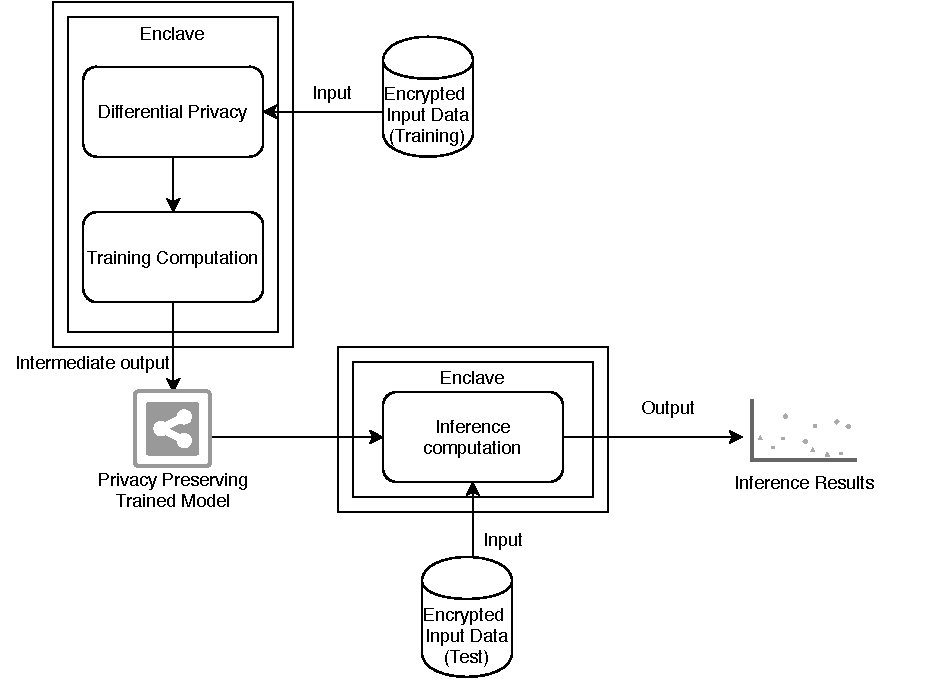
\includegraphics[width=10cm, height=10cm]{images/HLD.pdf}
    \caption{ High-level design}
    \label{fig:hld}
\end{figure}

\begin{itemize}
    \item \textbf{Differential privacy}
This module contains a mechanism to make the input training data differentially private to provide privacy on an individual's data. There are many perturbations techniques available to achieve differential privacy such as input, output, objective, and gradient perturbations. The perturbation techniques works by adding calibrated randomization over the input data before, during, or after the training. The randomization can be achieved using a randomized response technique or adding random noise from Laplace or Gaussian distribution. These noises are added in a way such that computations can be correctly performed and privacy of the data is also preserved \cite{3}. With this module, we will be enabling privacy property in our system SPML. To enable security property, SPML runs this module inside TEEs, which is Intel SGX in our case. 
    \vspace{-0.3cm}\item \textbf{Training computation}
This module is the main training computation module for training the model using the input dataset. The training can be either using machine learning or deep learning mechanisms. It is kind of a wrapper that can be called using APIs without changing much of the existing native machine learning code. This provides transparency and easy use of features for our SPML system. The training of the model takes place inside TEEs to prevent leakage of the trained model.
    \vspace{-0.3cm}\item \textbf{Inference computation}
 The real-world data on which inference is to be performed is kept in an encrypted form on the filesystem to protect its confidentiality and integrity. The user uploads the encrypted data and privacy-preserving trained model (i.e intermediate output of the training phase) in an untrusted environment and activates the inference computation module. The inference computation module performs computation to predict/classify the target output. All these computations take place inside TEEs protecting all the components always. The output of the inference is also saved in an encrypted form to prevent any kind of leakage.
\end{itemize}

Figure ~\ref{fig:hld} shows the high-level design of the SPML system. The workflow begins by uploading an encrypted training dataset to an untrusted enclave enabled cloud. SCONE runtime environment transparently decrypts the input dataset and bring this inside the enclave. The differential privacy module guarantees privacy via noise or randomized response. Depending upon the chosen DP technique corresponding DP module is activated. SPML system then starts training the model using the training computation module. This training can be either using machine learning or deep learning techniques. Both the differential privacy and training computation takes place inside an enclave hence their confidentiality and integrity of these modules are always protected. Training computation will produce a privacy-preserving trained model that will also be encrypted when outside the enclave. This marks the end of the training phase. The inference computation begins when some predictions/classification is to be done on real-word data using this trained model. The inference result will also be saved in an encrypted form when outside the enclave to protect its confidentiality and integrity.

\section{Design Detail}
In this section, the SPML design is explained in detail. The design is split into two phases (1) Training phase and (2) Inference phase. In both of these phases the computation happens inside the TEEs with the help of SCONE.
\begin{figure}
    \centering
    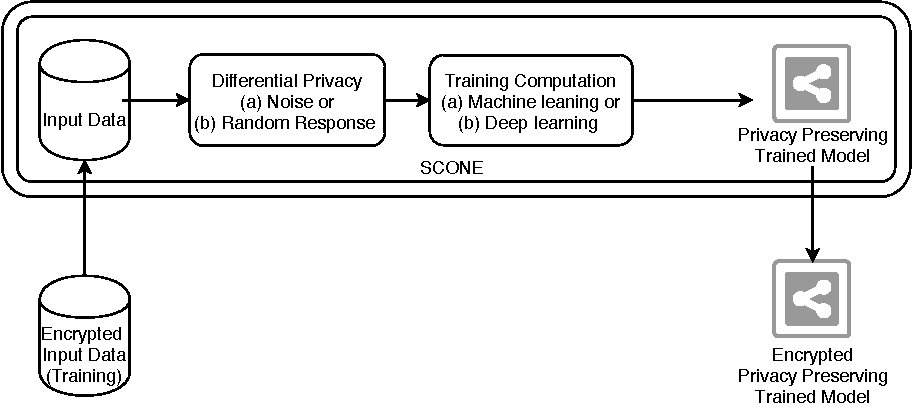
\includegraphics[width=\linewidth]{images/Training.pdf}
    \caption{Training phase}
    \label{fig:trainingDesign}
\end{figure}
\subsection{SCONE}
SCONE \cite{22} provides a platform that can help to build and securely run applications with any TEEs. TEEs provides confidentiality and integrity to the code and data by providing a secure execution region called as an enclave. Together with SCONE and TEEs data, model and code can be protected always. SCONE makes it achievable with minimum effort as there is no need to modify native existing application code. It means encryption/decryption required to protect data and code can be taken care of by SCONE. The secret keys required for encryption/decryption are supplied with the help of SCONE. SCONE has SCONE CAS(configuration and attestation service), which provides policy management and service attestation. The key generation is done inside TEE by SCONE CAS and is managed by a security policy (known as 'Session') of an application. The application code needs not to be changed, the injection of secrets can be done via configuration files or source files or compiled binaries on the TEE which is executing the application. Hence for applications, this process is transparent. SCONE not only gives us an efficient way to run applications within TEEs but it also does transparent encryption and decryption of files without changing the existing source code. SPML uses SCONE as a wrapper over the underlying TEEs (i.e Intel SGX in our case) for achieving confidentiality and integrity in the system.

\subsection{Training phase}
The training phase of our system SPML mainly focuses on training the model. The training is done with the help of the SCONE platform which provides execution in an encrypted manner. This means that data as well as the code are always in encrypted form. Clear text training data and code is only available to the application code. SCONE helps to simplify the encryption of an input, execution of application within the encrypted memory, and encryption of the output. Therefore, SCONE provides end to end transparent encryption/decryption by keeping data in always encrypted form during transmission, rest as well as processing. As shown in Figure ~\ref{fig:trainingDesign}, the input data is kept in an encrypted form on filesystem or harddisk. When computation needs to be performed the encrypted data is brought into the SCONE runtime environment which decrypts it and only application code which is SPML system modules can access that. This way the input data confidentiality and integrity are always protected.  Once the input dataset is decrypted, the privacy property is enabled by calling the differential privacy module.

\subsubsection{Differential privacy}
Differential privacy provides privacy to our system SPML. After choosing the technique of differential privacy that is randomized response or noise the next step is to make input data and model differentially private. If the randomized response is chosen which is our contribution to the SPML system, then the input dataset is made differentially private before training the model. The input dataset (full or some sensitive columns) is randomized using the probability bias p and q, where p is for the first coin flip, and q is for the second flip. The probability bias is the probability of getting the head \cite{14}. 

If noise is chosen then the input is submitted to the trained model and noise is added during the training of the model. For noise, the input dataset itself is not made differentially private but instead, noise is added during the training process in the objective or gradient functions. The noise here means a special type of calibrated random noise based on Gaussian or Laplace distribution. One needs to decide how much noise should be added so that the utility of the trained model is not degraded. If more noise is added then data becomes unusable hence there is always a trade-off between accuracy and utility. This notion is captured using the privacy budget concept as discussed below.

\textbf{Privacy Budget}
Differential privacy works by adding some noise at different levels of points such as before training on the data, during training on the model, or after training at the output. However, more noise means lesser accuracy hence there is always a trade-off to make between noise and accuracy level. This trade-off is defined in the form of mathematical calculation and is termed as $\epsilon$. Differential privacy calculates the privacy loss using this epsilon. There are different ways to calculate privacy loss depending upon the techniques used as follows:
\begin{itemize}
\item \textbf{Random response}
The randomized response works on a mechanism of a coin flip where the first coin is flipped with probability p and the second coin is flipped with probability q. These p and q are called bias, which are the probabilities of getting head. It provides $\epsilon$-\text{differential privacy}. To calculate epsilon and privacy loss for a randomized response, equations suggested in \cite{18} are used :
\begin{equation}
\epsilon = \log({\frac{p + (1 - p) * q}{(1 - p) * q}})
\label{eq:epsRR}
\end{equation}
Equation ~\ref{eq:epsRR} is used to calculate the epsilon value. For different p and q values, epsilon value differs and hence p and q can be used to control how much privacy or noise should be added.
\item \textbf{Noise}
Noise is added based on Gaussian Distribution or Laplace Distribution. Laplace satisfies $\epsilon$-\text{differential privacy} while Gaussian satisfies ($\epsilon$,$\delta$)-\text{differential privacy}. In our system SPML, we have used Gaussian noise and to calculate ($\epsilon$,$\delta$)-\text{differential privacy} the current method as discussed in equation ~\ref{eq:epsGaussian} is not an accurate fit, especially when composition with heterogeneous mechanisms is involved \cite{4} as in our system SPML. We will be using Rényi divergence to measure differential privacy based on paper \cite{23} which provides Rényi Differential Privacy (RDP), instead of using differential privacy in equation ~\ref{eq:epsGaussian}. SPML uses sampling distribution along with Gaussian noise and RDP is a perfect fit to calculate privacy when sampling is involved.
\end{itemize}
\subsubsection{Training Computation}
This is the module where the main machine learning computation happens. There are a lot of machine learning frameworks available to develop and train models such as Pytorch \cite{75}, Tensorflow \cite{24}, Scikit-learn library \cite{62}, etc. Depending upon the type of problem under consideration either machine learning or deep learning technique can be used. To train the differentially private model simple APIs are used like in the existing native machine learning/deep learning system with optimizers and loss functions. This computation takes place inside the SCONE and hence is secured even from the root user.

The training phase will produce a secure privacy-preserving trained model as shown in Figure ~\ref{fig:trainingDesign}. This model will not only protects confidentiality and integrity but also the privacy of the individuals. SCONE runtime environments encrypt this model before saving it to the filesystem. The encrypted trained model is used for inference by uploading it to the trusted environment when needed. The size of the model is usually small and hence it is easily portable and can be scaled up and down depending upon the demand providing easy portability and scalability. 
\begin{figure}
    \centering
    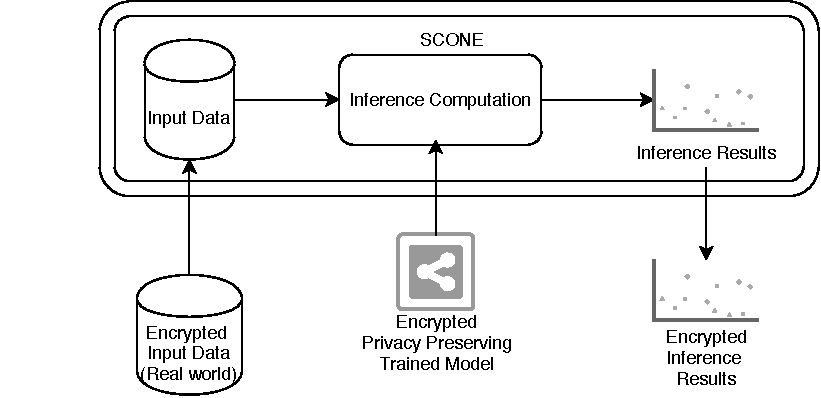
\includegraphics[width=\linewidth]{images/Inference.pdf}
    \caption{Inference phase}
    \label{fig:inferenceDesign}
\end{figure}
\subsection{Inference phase}
The inference phase of our system SPML means predicting/classifying on the trained model obtained from the last phase. The real-world data against which prediction/classification is to be made is also kept in an encrypted form in a filesystem. SCONE runtime environment is responsible for transparently decrypt it and provide clear text real-world data inside the enclave for inference. The real-world data is data that is not known to the previously trained model. This is the actual data of interest on which inference is required. As shown in Figure ~\ref{fig:inferenceDesign}, the input real-world data on which inference is to be made is fed into the inference computation module along with the trained model. This computation takes place inside the enclave, which means all the computation, model, and data are kept always encrypted in an untrusted environment. Inference computation involves correlating input data to predict/classify the output and coughing out the best possible outcome. \textbf{Encrypted inference result} will be the output of this phase and this is also encrypted by the SCONE runtime environment before saving it to the filesystem. Once, we have got the inference result, it marks the end of our system workflow.

\section{Summary}
Our system SPML provides privacy guarantees using differential privacy techniques to protect an individual's information. The confidentiality and integrity properties are enabled using TEE which in our case is Intel SGX. The SCONE runtime environment provides easy integration with TEEs. SCONE runtime environments take care of transparent encryption and decryption as well as make sure that all the data and computation happens inside the TEE. 

SPML consists of two phases training phase and the inference phase. In the training phase of SPML, we enable privacy property, and the model is trained with this property enabled. The privacy property is achieved using differential privacy and hence the trained model is privacy-preserving. By running SPML with TEEs security property gets enabled by default. With these two properties enabled, we can make any existing native machine learning system a secure privacy-preserving system. In the inference phase of SPML, we use a secure privacy-preserving model(i.e encrypted private model) obtained from the training phase to provide inference on real-world data. In this phase, also security property is enabled by default, hence inference results are always encrypted.

There are no changes required in the existing source code of the application and this helps us to fulfill our transparency goal. SCONE works in a docker like environment hence system can be easily scaled up and down on demand. SPML can be easily deployed in an untrusted enclave enabled cloud environment without the need to change anything. SCONE has very little overhead hence performance and accuracy are not much effected for the overall system. The SPML is designed in a way so that it fulfills all the discussed design goals. In the next chapter, we will discuss how we have implemented our system SPML.


\chapter{Implementation}
\label{sec:impl}
In this chapter, we will discuss how we have implemented SPML. We have chosen Intel SGX as TEEs and implemented our system with the help of the SCONE runtime environment due to the advantages it provides like transparency, containerization, easy deployment, etc. This chapter is divided into three sections. The first section discusses the differential privacy implementation details, followed by the implementation \footnote{https://github.com/prbh695a/SPML} details of the training and inference phase.
\section{Differential privacy}
In SPML, differential privacy is implemented based on the technique of adding calibrated random noise or randomized response. In practice, adding random noise to achieve differential privacy is a more preferred method than a randomized response. This is because in a randomized response each of the input data points is randomized and hence it changes overall data. However, in SPML we have implemented a randomized response as our contribution to study this effect. First, we will discuss how noise is implemented and then we will discuss implementation details of randomized response.

\subsection{Noise}
\label{sec:implementationNoise}
To run differential privacy with noise, Google provided privacy library \cite{11} based on start-of-the-art differential privacy paper for deep learning \cite{4}. This repository provides the \textit{tensorflow\_privacy} library which is developed in Python and can be used to train various machine learning models. This library contains implementation of various differentially private optimizers such as differentially private stochastic gradient descent, adam, adagrad, etc. \textit{tensorflow\_privacy} library can also be used with other python-based frameworks like PyTorch \cite{75}. Whether to train the model with the native optimizer using Google's TensorFlow or differential private optimizer can be easily controlled with the help of a flag as shown below :
\linebreak
\begin{lstlisting}[language=Python]
    if FLAGS.dpsgd:
        optimizer = DPGradientDescentGaussianOptimizer(
            l2_norm_clip=FLAGS.l2_norm_clip,
            noise_multiplier=noise,
            num_microbatches=FLAGS.microbatches,
            learning_rate=FLAGS.learning_rate)
        loss = K.losses.CategoricalCrossentropy(
            from_logits=True, reduction=tf.losses.Reduction.NONE)
    else:
        optimizer = GradientDescentOptimizer(learning_rate=FLAGS.learning_rate)
        loss = K.losses.CategoricalCrossentropy(from_logits=True, )
        model.compile(optimizer=optimizer, loss=loss, metrics=['accuracy'])
\end{lstlisting}
At Line1, FLAGS.dpsgd=true, then SPML will start training the model using differential private optimizers and loss function otherwise it will use the native TensorFlow functions. As we can see in above piece of code, that just by changing a few lines of code, any existing native machine learning algorithm can be made differentially private. Once we have obtained differential private model, we want to calculate privacy budget or privacy loss which is measured in terms of $\epsilon$.\newline
\newline
\textbf{Privacy Budget}
Privacy budget can be measured in terms of $\epsilon$ and $\delta$ where $\epsilon$ is the probability measure of how much privacy is being leaked and $\delta$ is a small probability of failing. But to calculate ($\epsilon$,$\delta$)-\text{differential privacy} with Gaussian and composition rule, the current method in equation ~\ref{eq:epsGaussian} is not an accurate fit. The \textit{tensorflow\_privacy} library recommends to use Rényi Differential Privacy (RDP) \cite{23}. Hence, we have used Rényi divergence to measure differential privacy which provides Rényi Differential Privacy (RDP). 

RDP enables us to calculate privacy when sampling distribution along with Gaussian noise is used like in our case. Tensorflow privacy library \cite{11} provides a function \textit{computeEpsilon()} to calculate epsilon based on hyperparameters such as dataset size, batch size, epochs, delta, and noise multiplier as explained below.
\begin{itemize}
    \item \textbf{Dataset size}: This is the size of the database or dataset.
    \vspace{-0.3cm}\item \textbf{Batch size}: Number of a random sample from the dataset which will be picked up during the training of model in each epoch.
    \vspace{-0.3cm}\item \textbf{Delta}: The $\delta$ should be set smaller then reciprocal of training data size.
    \vspace{-0.3cm}\item \textbf{Epoch}: Number of training iterations to train the model.
    \vspace{-0.3cm}\item \textbf{q} : It is the sampling ratio of number of samples in one step over total training samples. 
    \vspace{-0.3cm}\item \textbf{steps} : This is calculated as (Epoch * Dataset size) / (Batch size)
\end{itemize}

The function \textit{computeEpsilon()} as shown below can also be further integrated with any type of machine learning or deep learning mechanisms very easily. The advantage of this function is that it can be run independently of the training procedure and privacy loss can be obtained quickly and accurately at any point without training the model. Its a simple python script which doesn't have any dependency on any training or model parameters. 
\linebreak 
\begin{lstlisting}[language=Python]
def computeEpsilon(steps,noise):
  if noise == 0.0:
    return float('inf')
  orders = [1 + x / 10. for x in range(1, 100)] + list(range(12, 64))
  sampling_probability = FLAGS.batch_size / FLAGS.size
  rdp = compute_rdp(q=sampling_probability,
                    noise_multiplier=noise,
                    steps=steps,
                    orders=orders)
  return get_privacy_spent(orders, rdp, target_delta=FLAGS.delta)[0]
\end{lstlisting}
\subsection{Randomized response}
\label{sec:implementationRR}
In our system SPML, we have implemented the randomized response technique proposed by Warner \cite{14}. This technique is based on adding randomness to each person's response. The randomness is added by flipping a coin. For example, if simple questions are asked which can be answered in yes/no, then to answer these questions (1) A coined is flipped two times (2) If its head question is honestly answered (3) If its tail, then second coin flip comes into play and yes is answered for the head and no is answered for the tail. This provides plausible deniability because it cannot be traced if the answer is honestly answered or its due to the coin flip. The advantage of using this type of noise is that it is easy to implement but the major disadvantage is that, to add randomization each dataset must be studied and re-engineered/pre-processed to randomize it, which sometimes changes the overall dataset.
\linebreak
\begin{lstlisting}[language=Python]
def rr(column,p,q):
    for i in range(column.count()):
        flip1 = random.random() < p
        if flip1:
            continue
        else:
            flip2 = random.random() < q
            if flip2:
                column[i] = 1
            else:
                column[i] = 0
\end{lstlisting}
We have implemented our randomized response in a function \textit{rr}  based on simple coin flips. \textit{column} is the column in the dataset which will be randomized using this technique. \textit{p} and \textit{q} are called bias, which are the probabilities of getting head. The first coin is flipped with probability p and second coin with probability q. These p and q are used to calculate private budget for randomized response.\linebreak

\textbf{Privacy Budget}
To calculate epsilon and privacy loss, equations suggested in \cite{18} are used. The code for calculating the privacy budget is very simple as shown below. This function can also be used independently of any model parameters without starting the training process. In both the mechanisms, we can calculate the different parameters values to achieve the respective $\epsilon$.
\linebreak
\begin{lstlisting}[language=Python]
def calculateEps(p,q):
    numerator=(p+(1-p)*q)
    denominator=(1-p)*q
    eps=math.log(numerator/denominator)
    return eps
\end{lstlisting}
Once the user has decided which differential privacy technique to apply to activate privacy property i.e noise or randomized response, SPML can begin training our model depending upon the respective activated technique. 

\section{Training Phase}
For implementing the SPML system, there are many choices available to choose among the different machine learning frameworks such as Pytorch \cite{75}, Tensorflow \cite{24}, Scikit-learn library \cite{63}, etc. In SPML, Google's opensource framework TensorFlow is used to train models for machine/deep learning. It is known for its flexibility, wide range of libraries and community support to develop machine/deep learning applications. 

Tensorflow uses Python APIs for creating trained models. However, there are two known overheads when we use Python with SCONE. First is, python needs system call (dynamic library open (dlopen)) for import commands and this puts an additional overhead during integration with SCONE. The system call is responsible for loading libraries dynamically at run time in a program and is disabled by default. Secondly, python also requires setting large heap and stack sizes which degrades performance a little bit. To overcome these overheads, SCONE environment needs to be configured to allow the dlopen system call, heap, and stack size must be tuned to have a smooth run of an application.

\subsection{Training computation}
Training computation involves training the model with a native TensorFlow optimizer or differentially private optimizer. If we choose a randomized response then training will take place using native TensorFlow optimizers else differentially private optimizer. Training with differential private optimizer requires some additional parameters as compared to the existing hyperparameters as discussed below:
\begin{itemize}
    \item \textbf{learningRate}: The learning rate for the optimizer is the rate at which model learns in each iteration just like native TensorFlow. Since with differential privacy, the updates will be noisy hence this should be set as low for better training.
    \vspace{-0.3cm} \item \textbf{numMicrobatches}: The input data is usually split into batches in the native TensorFlow implementations, however, the differentially private optimizers requires the current batch to be split further into several micro-batches. Increasing the micro-batch tends to increase the utility but can slow down the training process hence a trade-off is required to make between utility and time taken for training. The batch size should be divisible by numMicrobatches else it results in an error.
    \vspace{-0.3cm} \item \textbf{l2NormClip}: This is the clip of the overall gradient of each micro-batch in a way such that the L2 norm of the gradient is maximum. This is set between .5 to 1.0.
    \vspace{-0.3cm} \item \textbf{noiseMultiplier}: It controls the noise amount to be added. Adding more noise can result in better privacy but will lower the accuracy. Here also a tradeoff between accuracy and privacy is required.
\end{itemize}

The training model, loss, and optimizer functions have been defined using python APIs in either case i.e native TensorFlow or differential privacy library. The main difference is how the model is trained using optimizer which can be native TensorFlow or from the privacy library. We will discuss details about how optimizers are made differentially private. In our discussion, we will be using Stochastic Gradient Descent(SGD) algorithm but this is applied in general to all other optimizers also. First, we will look into native SGD to understand how it works, then we will discuss the modification needed to make this native SGD into differentially private SGD.
\begin{itemize}
\item \textbf{Stochastic Gradient Descent}
Stochastic Gradient Descent (SGD) is an iterative algorithm. In this algorithm, random sample is picked from the training set, how many samples to be picked is decided by the batch size and they form a batch of data for every iteration. The loss is also known as an error and is computed between prediction done by the model and the labels, which undergoes a differentiation with parameters of the model. The resultant derivatives also known as gradients give an idea of how much each model parameters should be updated to reduce the error or loss to predict the correct training label. The decent comes from the recomputation of gradients and applying them to recalculate model's parameter. This process is repeated until the model is performing up to satisfaction. We summarized this process in steps as:
\begin{enumerate}
\item{A batch is picked up from the training points (x,y),where x stands for input and y stands for a label.}
\vspace{-0.3cm}\item{The loss function is defined as $L(theta, x, y)$ and is computed between the prediction of model f\_theta(x) and the label y, where theta stands for model's parameters.}
\vspace{-0.3cm}\item{Then, the gradient of this loss function is calculated using theta.}
\vspace{-0.3cm}\item{These gradients are then multiplied by learning rate and the product is applied to update theta.}
\end{enumerate}

\item \textbf{Differentially Private - Stochastic Gradient Descent}
Now we have looked and understood the basic working of SGD. To make SGD differentially private, two modifications are required. First, each gradient's sensitivity should be bounded. This is achieved by applying some limit on the training sample belonging to batch(es) so that they don't influence resultant gradient computation. It can be achieved within step3 and step4 by clipping gradient for every training point. Secondly, the algorithm behavior is randomized so that it is not possible to detect if a point was in the training set or not. To achieve this, random noise is sampled and added to the gradients which are clipped above. The final algorithm after modification will look like as follow:

\begin{enumerate}
\item{A batch is picked up from the training points (x,y), where x stands for input and y stands for a label.}
\vspace{-0.3cm}\item{Loss function is mathematically defined as $L(theta, x, y)$ and is computed between the prediction of model $f\_theta(x)$ and label y, theta stands for model's parameters.}
\vspace{-0.3cm}\item{Gradient of this loss function is calculated using theta.}
\vspace{-0.3cm}\item{These gradients are clipped over the batch so that each gradient is in Euclidean norm.}
\vspace{-0.3cm}\item{Random noise is added to each of these clipped gradients.}
\vspace{-0.3cm}\item{These noised and clipped gradients are then multiplied by learning rate and product is applied to update theta.}
\end{enumerate}

The algorithms which are either native TensorFlow or differentially private optimizers are called via python APIs as explained in section ~\ref{sec:implementationNoise}. Depending upon the chosen differentially private technique, a trained model will be obtained which will be privacy-preserving and will be encrypted via SCONE runtime environment and save for future use.
\end{itemize}

\section{Inference Phase}
Once the model is trained, it is ready to do prediction or classification for which it is trained. The trained model will try to co-relate the inputs to the best possible outcome to produce the output. The inference is required on some real-world data. The real-world data is the data on which model is not trained and hence is unknown to the model. Based on how accurate the inference is made for real-world data, the model accuracy can be estimated. Both the input data and the trained model are kept in an encrypted form in file-system to protect their confidentiality and integrity. When inference is required, the data and model will be run with a SCONE runtime environment which will transparently decrypt them and run computation over them within an enclave. \linebreak

\begin{lstlisting}[language=Python]
    modelName="Cifarmodel.h5"
    model = load_model("cifarmodelshwno/"+modelName)

    model.compile(optimizer=optimizer, loss=loss, metrics=['accuracy'])
    results = model.evaluate(test_data, test_labels, batch_size=FLAGS.batch_size)
\end{lstlisting}
The TensorFlow provides an API to load the saved model from the disk as explained in line1. We have to compile the model once again before doing inference. Line5 is evaluating a trained model against real-world data.

 The inference computation like training computation is also done inside the enclave using TensorFlow APIs. The inference is also known as the evaluation phase because this phase will determine how accurately the model can inference things and if this model can be used for real-time business cases. If the results of the inference phase are not satisfactory it means the model should be trained with more training data. Inference doesn't require setting large heap and stack size, unlike the training phase. Once inference is done, real-world data is not kept in memory. The result of the inference is also kept in encrypted form on a filesystem outside the SCONE.
\chapter{Evaluation}
\label{sec:eval}
In this chapter, SPML will be evaluated in terms of efficiency, accuracy, latency, and privacy. The details about the experimental setup used, the data set used, and the methodology followed will be discussed in this chapter. We have implemented Differential privacy using TensorFlow privacy library \cite{11} and randomized response. The TensorFlow privacy library adds random noise from Gaussian distribution during the model's training. The measurements will help us to understand the effect of adding differential privacy on a machine learning system in terms of latency and accuracy. The measurements will be carried on two popular machine learning public datasets MNIST \cite{12} and CIFAR10 \cite{13}. We have also run measurements to study the effect of adding randomized response which is our contribution to this framework. In the end, we have evaluated our system SPML against model inversion attack to show visually how image classification can be preserved and protected by enabling privacy and security property in our system.

\section{Experimental Setup}
To evaluate our system SPML for noise, Google's open-source TensorFlow privacy library is used. The repository \cite{11} contains a Python written library and can be used to train various machine learning models with differentially private TensorFlow optimizers such as differentially private stochastic gradient descent, adam, adagrad, etc. Additionally, it also provides tools to compute the privacy that will be achieved using these optimizers. TensorFlow privacy library version 0.2.2 was used as an underlying library to conduct measurements and TensorFlow version 1.15 was used with Keras version 2.3.1. 
\subsection{Testbed}
The machine used for running experiments was Linux with 2.2 GHz Quad-Core Intel(R) Xeon(R) CPU E3-1280 v6 @ 3.90GHz with 8 cores and RAM as 64 GB. 
\subsection{Methodology}
The measurements are classified into native TensorFlow (i.e SPML) and differential privacy (DP) run (i.e SPML+privacy). Native TensorFlow run means results are achieved with the optimizers from the native TensorFlow library \cite{46} and differential privacy run results are achieved with optimizers from the TensorFlow privacy library \cite{11}. To study the effect of enabling privacy feature in SPML on an existing machine learning system, we have executed DP (SPML+privacy) runs with six different values of epsilons 0.1, 1, 2, 4, 6, and 8. These measurements will help us to understand the relationship between different values of epsilon and accuracy as well as latency.

The native TensorFlow and DP run are conducted in three different environments (1) Native environment without SGX and SCONE (2) Simulation environment with SCONE, in a docker container, and without Intel SGX (3) Hardware environment with SCONE and Intel SGX, in a docker container. Even though docker containers are involved but the performance impact of docker on SPML is out of the scope of these measurements. In SPML, we want to evaluate the effect of enabling security and privacy property on accuracy and latency. To conclude this notion, each dataset will have a total of six experimental runs i.e native TensorFlow and DP run with three environments.

We will evaluate SPML for both of the phases of the machine learning system which are training and inference phase. Each phase will have six experiments as discussed above. For each phase, the final accuracy and latency score is an average of 10 iterations with 5 epochs for each epsilon value. In the next sections, the dataset and their evaluation are discussed.
\section{MNIST}
\label{sec:evalMnist}
The MNIST is a handwritten digits database \cite{12}. The original set has 60,000 training example but for this experiment, this dataset is reduced to use 10,000 examples for the training phase. These images are greyscaled and centered in a 28x28 image. For the inference phase, a dataset of 10,000 images from the original set is extracted and used for evaluating the trained model. Each of the pictures can be categorized as one of the digits from 0 to 9. For training the model, a convolutional neural network is used. It has two layers of convolution, each of this convolution layer follows a max-pooling layer. After these layers, a flatten layer is added followed by two dense layers. Both the Convolutional layers and one of the dense layer have rectified linear unit (ReLU ) activation function. These layers are connected using TensorFlow Python APIs. In the next subsections, training and inference results are discussed. 
\subsection{Training phase}
This subsection is organized into three parts as native mode, SCONE simulation mode, and SCONE hardware mode. In other words, we can say native mode means only enabling privacy property, SCONE hardware mode means enabling both privacy and security property. SCONE simulation mode gave us an idea about the overhead of running SPML in a SCONE runtime environment. For each mode, we will discuss the impact on accuracy and latency.

\subsubsection{Native Mode}
\begin{figure}
     \begin{subfigure}{0.5\textwidth}
         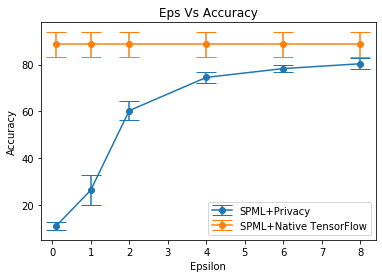
\includegraphics[width=\textwidth]{images/Training/MnistNativeAccuracy.png}
         \caption{Accuracy}
         \label{fig:nativeMnistAccuracyTraining}
     \end{subfigure}
     \begin{subfigure}{0.5\textwidth}
         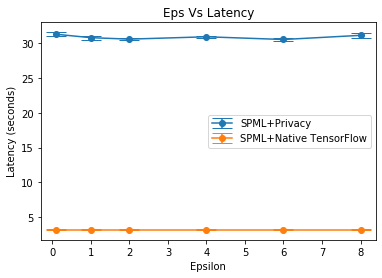
\includegraphics[width=\textwidth]{images/Training/MnistNativeLatency.png}
         \caption{Latency}
         \label{fig:nativeMnistLatencyTraining}
     \end{subfigure}
        \caption{MNIST Dataset - Training - Native mode without Intel SGX and SCONE}
     \begin{subfigure}{0.5\textwidth}
         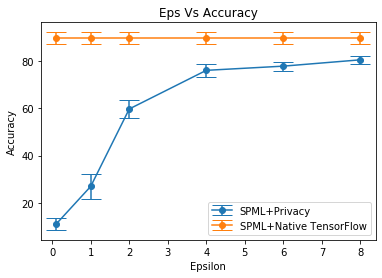
\includegraphics[width=\textwidth]{images/Training/MnistSimAccuracy.png}
         \caption{Accuracy}
         \label{fig:simMnistAccuracyTraining}
     \end{subfigure}
     \begin{subfigure}{0.5\textwidth}
         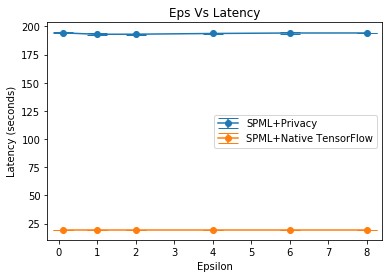
\includegraphics[width=\textwidth]{images/Training/MnistSimLatency.png}
         \caption{Latency}
         \label{fig:simMnistLatencyTraining}
     \end{subfigure}
        \caption{MNIST Dataset - Training - Simulation mode without Intel SGX and with SCONE}
     \begin{subfigure}{0.5\textwidth}
         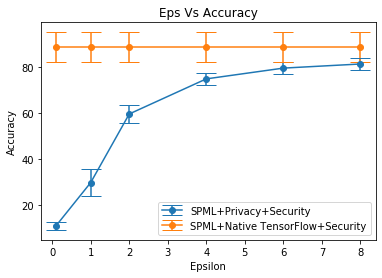
\includegraphics[width=\textwidth]{images/Training/MnistHWAccuracy.png}
         \caption{Accuracy}
         \label{fig:hwMnistAccuracyTraining}
     \end{subfigure}
     \begin{subfigure}{0.5\textwidth}
         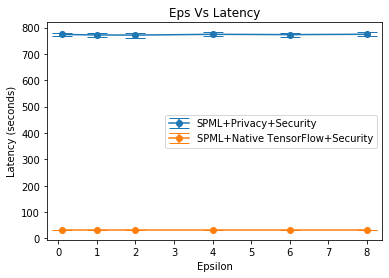
\includegraphics[width=\textwidth]{images/Training/MnistHWLatency.png}
         \caption{Latency}
         \label{fig:hwMnistLatencyTraining}
     \end{subfigure}
        \caption{MNIST Dataset - Training - Hardware mode with Intel SGX and SCONE}
\end{figure}
\begin{figure}
     \begin{subfigure}{0.5\textwidth}
         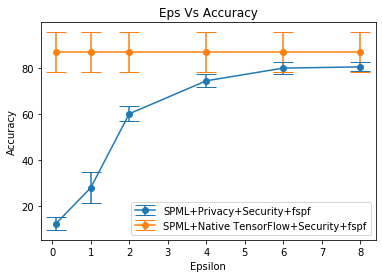
\includegraphics[width=\textwidth]{images/Training/MnistHWFSPFAccuracy.png}
         \caption{Accuracy}
         \label{fig:fspfMnistAccuracyTraining}
     \end{subfigure}
     \begin{subfigure}{0.5\textwidth}
         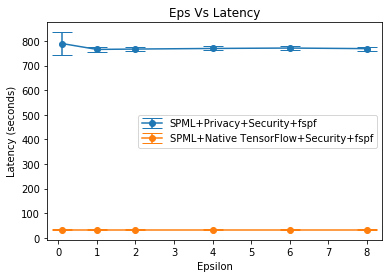
\includegraphics[width=\textwidth]{images/Training/MnistHWFSPFLatency.png}
         \caption{Latency}
         \label{fig:fspfMnistLatencyTraining}
     \end{subfigure}
        \caption{MNIST Dataset - Training - Hardware mode + Fspf with Intel SGX and SCONE}
\end{figure}
\textbf{\textit{Accuracy: }}The accuracy here means the rate at which we predict or classify the correct data out of the whole set. Figure ~\ref{fig:nativeMnistAccuracyTraining} shows the native mode measurements of the MNIST dataset for accuracy. The SPML+native TensorFlow run achieved accuracy of 88\%. SPML+Privacy runs shows an increasing trend from epsilon value 0.1 to 8. With epsilon value 0.1, only accuracy of 11\% is achieved. The accuracy kept on increasing as epsilon value is increased and accuracy of 80\% is achieved at epsilon value 8. This is because as we increase the epsilon value the noise level decreases, hence accuracy value should increase. This notion is clearly shown in Figure ~\ref{fig:nativeMnistAccuracyTraining}. Hence, we can say that at smaller epsilon values we protect strongly, but this will lead to some degradation in accuracy. This is always a trade-off to decide at what level we need protection and accuracy.
\newline
\newline
\textbf{\textit{Latency: }}The Figure ~\ref{fig:nativeMnistLatencyTraining} shows the native mode measurements of the MNIST dataset for latency. The SPML+native TensorFlow run shows the latency of 3 seconds. All the SPML+Privacy runs for different values of epsilons show almost the same latency value of 30 seconds. This means latency doesn't change much with different epsilon values. The SPML+Privacy runs have almost 10$\times$ latency as compare to SPML+native TensorFlow runs. Hence, we can say that this is the approximation cost in terms of latency for adding privacy property into our system SPML. Next, we will look into the accuracy and latency values for running SPML in SCONE runtime environment.


\subsubsection{SCONE simulation mode}
\textbf{\textit{Accuracy: }} In SCONE simulation mode, the accuracy trend as explained above remains the same. As in the previous measure of SPML in native mode (i.e without Intel SGX and SCONE), we have seen that accuracy increases as epsilon value increases. Figure ~\ref{fig:simMnistAccuracyTraining} shows the epsilon value of 0.1 achieves an accuracy of 10\% and the epsilon value of 8 achieves an accuracy of 80\%. The accuracy trend in SCONE simulation mode for SPML+Privacy and SPML+native TensorFlow run is almost the same as the native (i.e without Intel SGX and SCONE) mode run. Hence, we can say that simulation mode has very little or no effect on accuracy.
\begin{table}[h!]
  \begin{center}
    \caption{MNIST Latency Comparison - Training }
    \label{tab:mnistLatencyTraining}
    \begin{tabular}{|c|c|c|}
      \hline
      \textbf{} & \textbf{SPML +} & \textbf{SPML +} \\
      \textbf{} & \textbf{native TensorFlow} & \textbf{privacy} \\
      \textbf{} & \textbf{(seconds)} & \textbf{(seconds)} \\
      \hline
      \textbf{Native mode} & 3        &   30\\
      \hline
      \textbf{SCONE simulation mode} &  19       &     195\\
      \hline    
      \textbf{SCONE hardware mode} &    32     &      775\\
      \hline
    \end{tabular}
   \end{center}
\end{table}
\newline
\newline
\textbf{\textit{Latency: }}The latency of SPML as shown in ~\ref{fig:simMnistLatencyTraining} remains almost constant for all epsilon value around 195 seconds and the SPML+native TensorFlow run has a latency of around 19 seconds. The table ~\ref{tab:mnistLatencyTraining} shows quick comparison of latency for all modes. The latency for simulation mode is 6$\times$ times higher as compared to the native(i.e without Intel SGX and SCONE) mode for SPML+Privacy and SPML+native TensorFlow run. This means this is the cost of enabling privacy property in SPML in SCONE simulation mode. In the next experiment, we want to evaluate security property in SCONE hardware mode.

\subsubsection{SCONE hardware mode}
The hardware mode means running SPML with Intel SGX and SCONE environment. SCONE FSPF \cite{77} is needed to transparently encrypt/decrypt the data, code, and model. SCONE FSPF perform cryptography related operation using Intel-CPU-specific hardware instructions. In this section, we have evaluated our system SPML for both choices, if we enable file system shield (i.e FSPF) and if we don't enable this shield (i.e without FSPF). It should not make any difference if we run SPML with FSPF and without FSPF as measurement should be ideally the same for both of these options. We will be discussing results for both the choices in next paragraph.
\newline
\newline
\textbf{\textit{Accuracy: }} In SCONE hardware mode also, the accuracy trend remains the same. As seen in the previous measurement of the accuracy of SPML in native and simulation mode, we have seen that accuracy increases as epsilon value increases. Figure ~\ref{fig:hwMnistAccuracyTraining}, ~\ref{fig:fspfMnistAccuracyTraining} shows that the accuracy trends increase from 10 to 80 \% for 0.1 and 8 epsilon value respectively without and with FSPF. Hence this shows that the accuracy trend in SCONE hardware mode(with FSPF and without FSPF) for SPML+privacy and SPML+native TensorFlow run is almost the same as native or simulation mode run. Hence, we can say that hardware mode has very little or no effect on the accuracy of SPML like SCONE simulation mode.
\newline 
\newline
\textbf{\textit{Latency: }}The latency as shown in Figure ~\ref{fig:hwMnistLatencyTraining}, ~\ref{fig:fspfMnistLatencyTraining} remain almost constant for all epsilon value around 775 seconds with SPML+privacy run without and with FSPF. On the other hand, the SPML+native TensorFlow run has a latency of around 38 seconds. Hardware mode means security is enabled by default. So we can say the SPML system is SPML + security. As shown in Table ~\ref{tab:mnistLatencyTraining}, SPML+security+privacy has 24$\times$ latency as compared to SPML+security without privacy. The latency for hardware mode is 4$\times$, 25$\times$ times higher as compared to simulation, and the native mode for SPML+security+privacy respectively. The SPML+security without privacy run has latency almost 1.5$\times$, 10.5$\times$ as compare to the SPML without privacy run in simulation and native mode respectively.

For hardware mode, the training accuracy and latency trends with FSPF and without FSPF are almost the same. It means transparent encryption/decryption by SCONE for code, data and model are not adding any overhead in terms of latency and accuracy. We have run FSPF mode only for the MNIST dataset to conclude this notion.

It is seen that hardware mode, which is enabling security property in our system SPML, has very high latency. The reason for this is the small EPC size, where code, data, and model are executed. The EPC size is 90MB and the classification process usually takes 330MB of main memory and the process is independent of training size (i.e number of images) \cite{81}. Therefore, paging is required as EPC memory is exceeded during this process, which is achieved using page swap to non-encrypted main memory. To protect the data again after swapping, the encryption process needs to be repeated. Hence this leads to the poor performance of read and writes, and degrades overall performance in terms of latency.

However, on the other hand, privacy, confidentiality, and integrity are also added on code, data, and model. Hence we can say that this is the cost in terms of latency one needs to take for training the models. The good thing is that in practice, we can perform training over the weekend or as nightly run to save efforts and time for developers. Hence this extra latency can be avoided and dealt with if planned well in advance. However, the inference is used more frequently to predict or classify, so it should have latency within reasonable limits so that our SPML system can be used in the normal office working hours. In the next section, we want to evaluate the SPML system for the inference phase.
\subsection{Inference phase}
This subsection is organized into two parts as accuracy and latency and all three modes are discussed.
\begin{figure}
     \begin{subfigure}{0.5\textwidth}
         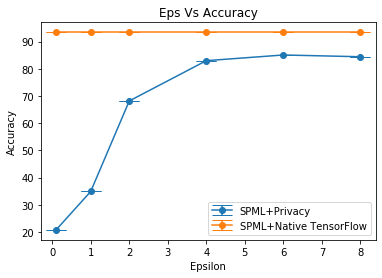
\includegraphics[width=\textwidth]{images/Inference/MnistNativeAccuracyInference.png}
         \caption{Accuracy}
         \label{fig:nativeMnistAccuracyInference}
     \end{subfigure}
     \begin{subfigure}{0.5\textwidth}
         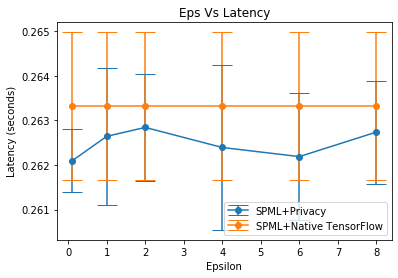
\includegraphics[width=\textwidth]{images/Inference/MnistNativeLatencyInference.png}
         \caption{Latency}
         \label{fig:nativeMnistLatencyInference}
     \end{subfigure}
        \caption{MNIST Dataset - Inference - Native mode without Intel SGX and SCONE}
     \begin{subfigure}{0.5\textwidth}
         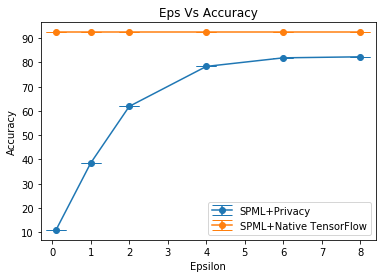
\includegraphics[width=\textwidth]{images/Inference/MnistSimAccuracyInference.png}
         \caption{Accuracy}
         \label{fig:simMnistAccuracyInference}
     \end{subfigure}
     \begin{subfigure}{0.5\textwidth}
         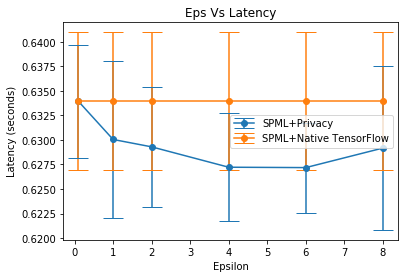
\includegraphics[width=\textwidth]{images/Inference/MnistSimLatencyInference.png}
         \caption{Latency}
         \label{fig:simMnistLatencyInference}
     \end{subfigure}
        \caption{MNIST Dataset - Inference - Simulation mode without Intel SGX and with SCONE}
     \begin{subfigure}{0.5\textwidth}
         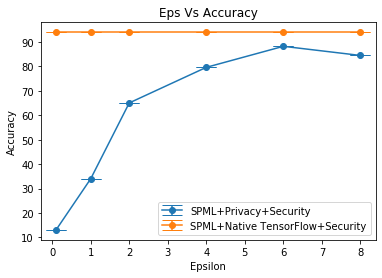
\includegraphics[width=\textwidth]{images/Inference/MnistHwAccuracyInference.png}
         \caption{Accuracy}
         \label{fig:hwMnistAccuracyInference}
     \end{subfigure}
     \begin{subfigure}{0.5\textwidth}
         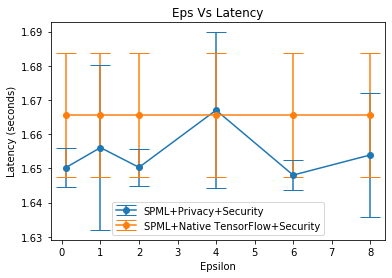
\includegraphics[width=\textwidth]{images/Inference/MnistHwLatencyInference.png}
         \caption{Latency}
         \label{fig:hwMnistLatencyInference}
     \end{subfigure}
        \caption{MNIST Dataset - Inference - Hardware mode with Intel SGX and SCONE}
\end{figure}
\begin{figure}
     \begin{subfigure}{0.5\textwidth}
         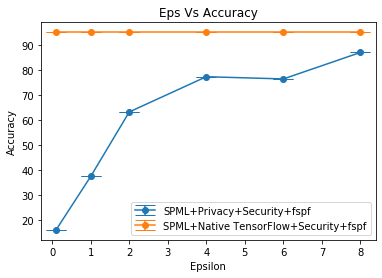
\includegraphics[width=\textwidth]{images/Inference/MnistFSPFAccuracyInference.png}
         \caption{Accuracy}
         \label{fig:fspfMnistAccuracyInference}
     \end{subfigure}
     \begin{subfigure}{0.5\textwidth}
         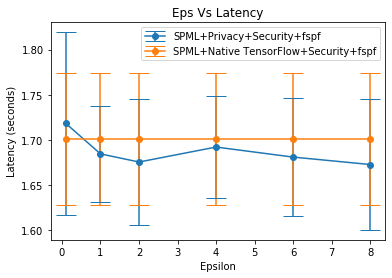
\includegraphics[width=\textwidth]{images/Inference/MnistFSPFLatencyInference.png}
         \caption{Latency}
         \label{fig:fspfMnistLatencyInference}
     \end{subfigure}
        \caption{MNIST Dataset - Inference - Hardware mode + Fspf with Intel SGX and SCONE}
\end{figure}
\newline
\newline
\textbf{\textit{Accuracy: }}The inference figures of accuracy for native, simulation, and hardware mode without and with FSPF are shown in Figure ~\ref{fig:nativeMnistAccuracyInference}, ~\ref{fig:simMnistAccuracyInference}, ~\ref{fig:hwMnistAccuracyInference}, ~\ref{fig:fspfMnistAccuracyInference}  respectively. Accuracy depends upon the model that is being trained and used for doing inference. If the model trained and saved have good accuracy then inferences have good accuracy. Inference accuracy in all three modes is almost the same for example the SPML+native TensorFlow model is giving an accuracy of around 94\% and the hardware is giving an accuracy of around 93.98\%. Hence accuracy in the inference phase also remains nearly comparable to the native environment and the accuracy trend remains the same which is accuracy increases as epsilon value increases.
\newline
\newline
\textbf{\textit{Latency: }}The inference figures of latency for native, simulation, and hardware mode without and with FSPF are shown in Figure ~\ref{fig:nativeMnistLatencyInference}, ~\ref{fig:simMnistLatencyInference}, ~\ref{fig:hwMnistLatencyInference}, ~\ref{fig:fspfMnistLatencyInference} respectively. The figures show that the time taken for inference is almost the same for differentially private as well as native TensorFlow algorithms. The inference has less effect in terms of whether the model is trained with differential privacy or native TensorFlow. The time taken for inference is also very less as compared to the time taken in training the models. For example, in hardware mode (SPML+Privacy+Security) inference takes around 1.66 seconds while training takes around 775 seconds and there is a huge difference between the time taken for training and inference. \newline
\begin{table}[h!]
  \begin{center}
    \caption{MNIST Latency Comparison - Inference }
    \label{tab:mnistLatencyInference}
    \begin{tabular}{|c|c|c|}
      \hline
      \textbf{} & \textbf{SPML +} & \textbf{SPML +} \\
      \textbf{} & \textbf{native TensorFlow} & \textbf{privacy} \\
      \textbf{} & \textbf{(seconds)} & \textbf{(seconds)} \\
      \hline
      \textbf{Native mode} & .26        &   .26\\
      \hline
      \textbf{SCONE simulation mode} &  .63       &     .63\\
      \hline    
      \textbf{SCONE hardware mode} &    1.66     &      1.66\\
      \hline
    \end{tabular}
   \end{center}
\end{table}
As shown in table ~\ref{tab:mnistLatencyInference}, the native (i.e without Intel SGX and SCONE) mode is completed within 0.26 seconds and hardware (i.e with Intel SGX and SCONE) takes around 1.66 seconds. Hardware mode has, 6.3$\times$ latency as compared to native and 2.63$\times$ than simulation mode respectively. The simulation mode has 2.4$\times$ latency as compared to native mode for both SPML+native Tensorflow and SPML+Privacy runs. Hence, inference doesn't increase a lot of computational overhead in terms of latency for simulation or hardware mode. There is some overhead but it is within acceptable limits to use it in practice. Next, we have evaluated the Cifar10 dataset results to study and understand if we can draw the same conclusion with this dataset also.

\section{Cifar10}
\label{sec:evalCifar10}
The Cifar10 database\cite{13} has 60000 32x32 training images. These images belong to 10 classes such as airplanes, automobiles, birds, etc. For training the model convolutional neural network is used. It has three layers of convolution, first two convolution layer follows a max pooling layer. After these layers, a flatten layer is added followed by two dense layers. Both the convolutional layers and one of the dense layer have rectified linear unit (ReLU ) activation function. These all layers are connected together using TensorFlow Python APIs. In the next subsections, training and inference results are discussed.
\subsection{Training phase}
\textbf{\textit{Accuracy: }} The notion of accuracy which we saw in the last section is same for this dataset also. The accuracy trend increases with epsilon value in all three modes. As can be seen in Figure ~\ref{fig:nativeCifar10AccuracyTraining}, ~\ref{fig:simCifar10AccuracyTraining}, ~\ref{fig:hwCifar10AccuracyTraining} for all modes, accuracy starts from around 10\% and goes upto 15\% at 0.1 and 8 epsilon value respectively. Hence it is true for this dataset also that accuracy is effected very little by the environment or the mode.
\begin{figure}
     \begin{subfigure}{0.5\textwidth}
         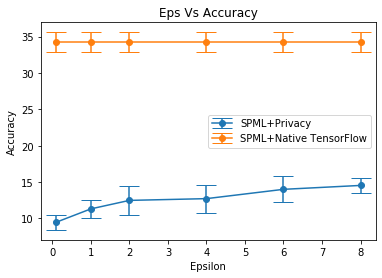
\includegraphics[width=\textwidth]{images/Training/Cifar10NativeAccuracy.png}
         \caption{Accuracy}
         \label{fig:nativeCifar10AccuracyTraining}
     \end{subfigure}
     \begin{subfigure}{0.5\textwidth}
         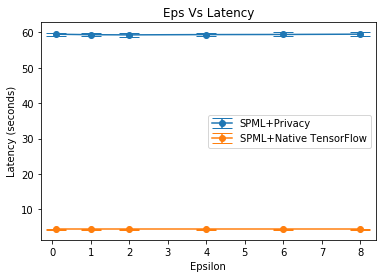
\includegraphics[width=\textwidth]{images/Training/Cifar10lNativeLatency.png}
         \caption{Latency}
         \label{fig:nativeCifar10LatencyTraining}
     \end{subfigure}
        \caption{Cifar10 Dataset - Training - Native mode without Intel SGX and SCONE}
     \begin{subfigure}{0.5\textwidth}
         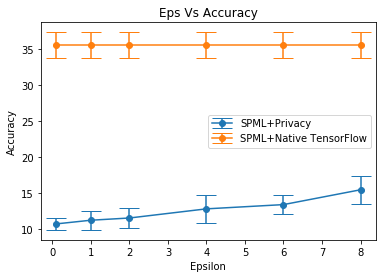
\includegraphics[width=\textwidth]{images/Training/Cifar10SimAccuracy.png}
         \caption{Accuracy}
         \label{fig:simCifar10AccuracyTraining}
     \end{subfigure}
     \begin{subfigure}{0.5\textwidth}
         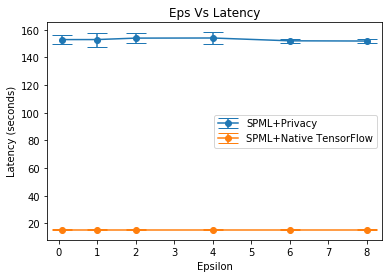
\includegraphics[width=\textwidth]{images/Training/Cifar10SimLatency.png}
         \caption{Latency}
         \label{fig:simCifar10LatencyTraining}
     \end{subfigure}
        \caption{Cifar10 Dataset - Training - Simulation mode without Intel SGX and with SCONE}
     \begin{subfigure}{0.5\textwidth}
         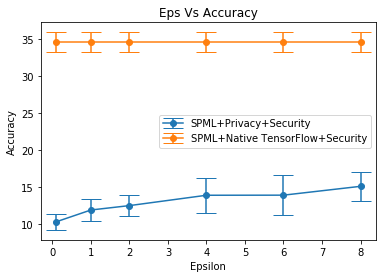
\includegraphics[width=\textwidth]{images/Training/Cifar10HWAccuracy.png}
         \caption{Accuracy}
         \label{fig:hwCifar10AccuracyTraining}
     \end{subfigure}
     \begin{subfigure}{0.5\textwidth}
         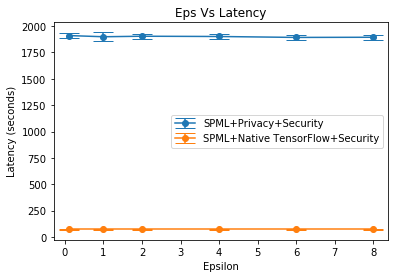
\includegraphics[width=\textwidth]{images/Training/Cifar10HWLatency.png}
         \caption{Latency}
         \label{fig:hwCifar10LatencyTraining}
     \end{subfigure}
        \caption{Cifar10 Dataset - Training - Hardware mode with Intel SGX and SCONE}
\end{figure}
\newline
\newline
\textbf{\textit{Latency: }}The latency graphs for this dataset are shown in Figure ~\ref{fig:nativeCifar10LatencyTraining}, ~\ref{fig:simCifar10LatencyTraining}, ~\ref{fig:hwCifar10LatencyTraining}. Latency doesn't increase or decrease much with the epsilon values. However, the latency of native vs simulation vs hardware mode has huge gap among themselves. The hardware mode (SPML+security+privacy) latency for Cifar10 dataset is 2030 seconds which is almost 13.35$\times$, 34.4$\times$ as compared to simulation(152 seconds) and native (59 seconds) mode latency for DP(SPML+privacy) run respectively. For native TensorFlow run(SPML+native TensorFlow), the hardware mode (SPML+security) latency is 5$\times$, 18.75$\times$ as compared to simulation and native mode latency. Hence, it can be concluded that hardware mode adds some overhead for latency for our system SPML, but at the same time we are getting a trained privacy preserving secure model. As discussed above, these latency can be tolerated and training can be planned using overnight or over weekends to save time. We evaluated inference results also to see if these can be used in practise like MNIST dataset.

\subsection{Inference phase}
\textbf{\textit{Accuracy: }} The figures ~\ref{fig:nativeCifar10AccuracyInference}, ~\ref{fig:simCifar10AccuracyInference}, ~\ref{fig:hwCifar10AccuracyInference} shows the accuracy trend for the Cifar10 dataset for inference for all the three modes. The native TensorFlow accuracy for all the modes remains the same between 9-10 \%. Since we used only 3000 images for training the model, hence for all epsilon values the same kind of inference trend is shown. With these result, it can be concluded that accuracy of native vs simulation vs hardware mode remains almost same and inference accuracy like training is not much affected by the environment.
\begin{figure}
     \begin{subfigure}{0.5\textwidth}
         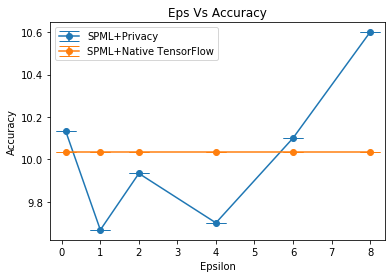
\includegraphics[width=\textwidth]{images/Inference/Cifar10NativeAccuracyInference.png}
         \caption{Accuracy}
         \label{fig:nativeCifar10AccuracyInference}
     \end{subfigure}
     \begin{subfigure}{0.5\textwidth}
         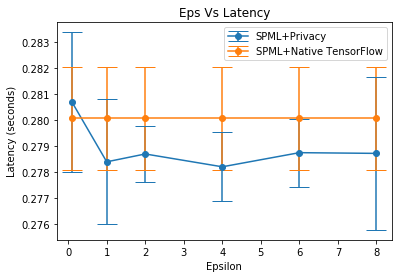
\includegraphics[width=\textwidth]{images/Inference/Cifar10NativeLatencyInference.png}
         \caption{Latency}
         \label{fig:nativeCifar10LatencyInference}
     \end{subfigure}
        \caption{Cifar10 Dataset - Inference - Native mode without Intel SGX and SCONE}
     \begin{subfigure}{0.5\textwidth}
         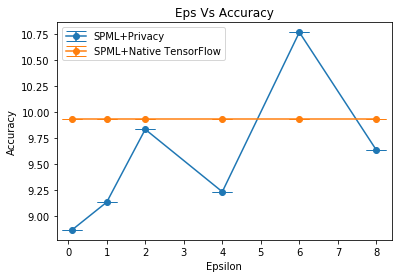
\includegraphics[width=\textwidth]{images/Inference/Cifar10SimAccuracyInference.png}
         \caption{Accuracy}
         \label{fig:simCifar10AccuracyInference}
     \end{subfigure}
     \begin{subfigure}{0.5\textwidth}
         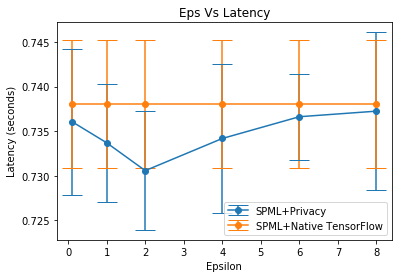
\includegraphics[width=\textwidth]{images/Inference/Cifar10SimLatencyInference.png}
         \caption{Latency}
         \label{fig:simCifar10LatencyInference}
     \end{subfigure}
        \caption{Cifar10 Dataset - Inference - Simulation mode without Intel SGX and with SCONE}
     \begin{subfigure}{0.5\textwidth}
         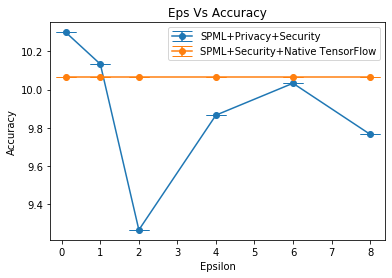
\includegraphics[width=\textwidth]{images/Inference/Cifar10HwAccuracyInference.png}
         \caption{Accuracy}
         \label{fig:hwCifar10AccuracyInference}
     \end{subfigure}
     \begin{subfigure}{0.5\textwidth}
         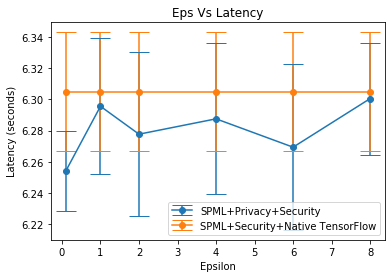
\includegraphics[width=\textwidth]{images/Inference/Cifar10HwLatencyInference.png}
         \caption{Latency}
         \label{fig:hwCifar10LatencyInference}
     \end{subfigure}
        \caption{Cifar10 Dataset - Inference - Hardware mode with Intel SGX and SCONE}
\end{figure}
\newline
\newline
\textbf{\textit{Latency: }}The figures ~\ref{fig:nativeCifar10LatencyInference}, ~\ref{fig:simCifar10LatencyInference}, ~\ref{fig:hwCifar10LatencyInference} shows the inference latency of all the modes. There is not much difference between the latency of the native TensorFlow (SPML) and DP (SPML+privacy) run. However, hardware mode (SPML+security) is almost showing latency of 5.9 seconds which is 7.5$\times$, 19$\times$ as compared to simulation and native mode (SPML without security) respectively. These latency values are much less than the latency of the training phase. Hence, the inference phase can be used in practice because latency is within an acceptable range. 

\section{Randomized response}
To evaluate the randomized response technique for our system SPML, we have used adult dataset \cite{15}. It contains census data with attributes like age, education, relationship, sex, occupation, etc and using these attributes it predicts if the income of an individual can exceed \$50000/year. We choose the sex and relationship column and made them numerical with 0 or 1 responses. Then we added randomization to this dataset by randomizing the sex and relationship numerical column with the coin flip algorithm as explained in the implementation section ~\ref{sec:implementationRR}. We trained the model on 39040 training samples and 9792 inference samples. We followed the same methodology as explained above but the only difference is we used different epoch values for this such as 0.13, 0.53, 1, 2, 3, 4. For each phase, the final accuracy and latency score is an average of 10 iterations with 50 epochs for each epsilon value. In the next sections, we will discuss the results we got from the training and inference phase.

\subsection{Training Phase}
\textbf{\textit{Accuracy: }} As we can see from Figures ~\ref{fig:nativeRRAccuracyTraining}, ~\ref{fig:simRRAccuracyTraining}, ~\ref{fig:hwRRAccuracyTraining} accuracy fluctuates a lot for each epsilon value. It is hard to conclude any trend, like with noise, we can say that accuracy increases with epsilon value. The accuracy with randomized response, remains between 72\% to 75\%. We get definitely almost comparable accuracy as compared to native TensorFlow in all three modes however no trend can be established between accuracy and espilon value.
\begin{figure}
     \begin{subfigure}{0.5\textwidth}
         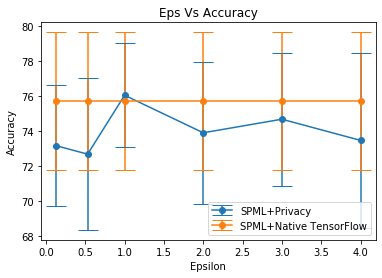
\includegraphics[width=\textwidth]{images/Training/RRAccuracy.png}
         \caption{Accuracy}
         \label{fig:nativeRRAccuracyTraining}
     \end{subfigure}
     \begin{subfigure}{0.5\textwidth}
         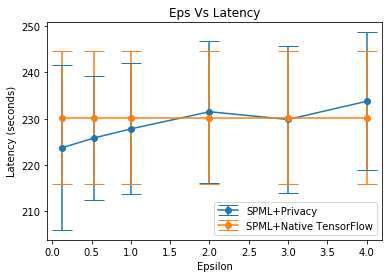
\includegraphics[width=\textwidth]{images/Training/RRLatency.png}
         \caption{Latency}
         \label{fig:nativeRRLatencyTraining}
     \end{subfigure}
        \caption{Randomized response - Training - Native mode without Intel SGX and SCONE}
     \begin{subfigure}{0.5\textwidth}
         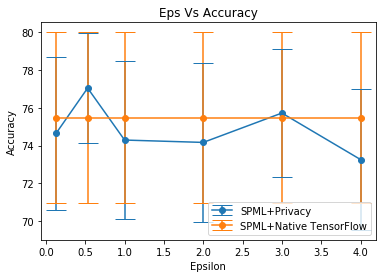
\includegraphics[width=\textwidth]{images/Training/RRSIMAccuracy.png}
         \caption{Accuracy}
         \label{fig:simRRAccuracyTraining}
     \end{subfigure}
     \begin{subfigure}{0.5\textwidth}
         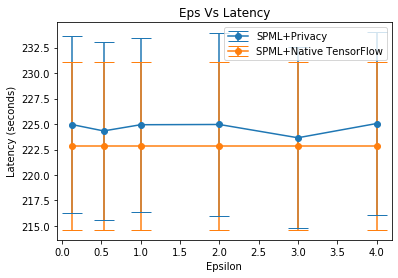
\includegraphics[width=\textwidth]{images/Training/RRSIMLatency.png}
         \caption{Latency}
         \label{fig:simRRLatencyTraining}
     \end{subfigure}
        \caption{Randomized response - Training - Simulation mode without Intel SGX and with SCONE}
        \label{default}
     \begin{subfigure}{0.5\textwidth}
         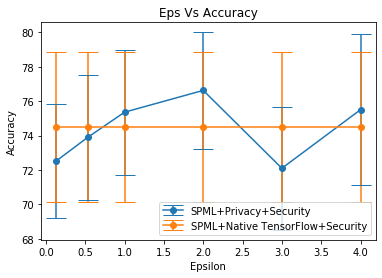
\includegraphics[width=\textwidth]{images/Training/RRHWAccuracy.png}
         \caption{Accuracy}
         \label{fig:hwRRAccuracyTraining}
     \end{subfigure}
     \begin{subfigure}{0.5\textwidth}
         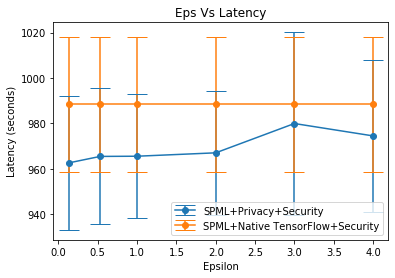
\includegraphics[width=\textwidth]{images/Training/RRHWLatency.png}
         \caption{Latency}
         \label{fig:hwRRLatencyTraining}
     \end{subfigure}
        \caption{Randomized response - Training - Hardware mode with Intel SGX and SCONE}
\end{figure}
\newline
\newline
\textbf{\textit{Latency: }}We can see the Figures in ~\ref{fig:nativeRRLatencyTraining}, ~\ref{fig:simRRLatencyTraining}, ~\ref{fig:hwRRLatencyTraining} for native, simulation, and hardware modes respectively. There is not much difference between native Tensorflow(SPML) and DP(SPML+privacy) run in terms of latency. SPML without privacy and SPML+privacy both have a latency of around 225, 225, 965 seconds for native, simulation, and hardware mode respectively. SPML has a latency of around 225 seconds for native and simulation mode while SPML + security is touching latency of around 965 seconds. After enabling security property in SPML latency is almost 4.2$\times$ as compared to SPML without security.
\subsection{Inference Phase}
\textbf{\textit{Accuracy: }} We can see that accuracy fluctuates a lot for each epsilon value in our system SPML for inference also as can be seen in Figures ~\ref{fig:nativeRRAccuracyInference}, ~\ref{fig:simRRAccuracyInference}, ~\ref{fig:hwRRAccuracyInference} . As discussed in the training phase, it is hard to conclude any trend here. The accuracy values are between 80\% and 82\%. We get definitely almost comparable accuracy as compared to native TensorFlow in all three modes however no trend can be established between accuracy and epsilon value.
\begin{figure}
     \begin{subfigure}{0.5\textwidth}
         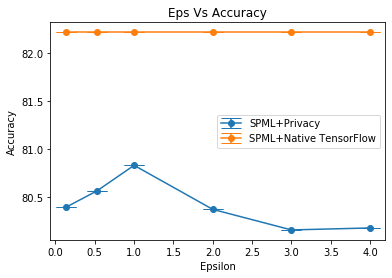
\includegraphics[width=\textwidth]{images/Inference/RRAccuracy.png}
         \caption{Accuracy}
         \label{fig:nativeRRAccuracyInference}
     \end{subfigure}
     \begin{subfigure}{0.5\textwidth}
         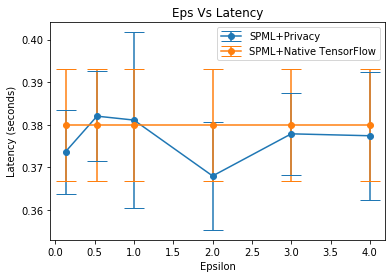
\includegraphics[width=\textwidth]{images/Inference/RRLatency.png}
         \caption{Latency}
         \label{fig:nativeRRLatencyInference}
     \end{subfigure}
        \caption{Randomized response - Inference - Native mode without Intel SGX and SCONE}
     \begin{subfigure}{0.5\textwidth}
         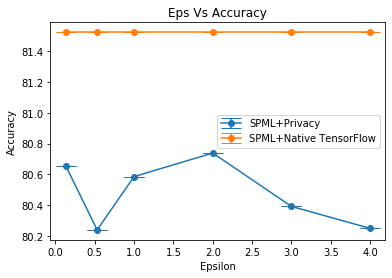
\includegraphics[width=\textwidth]{images/Inference/RRSIMAccuracy.png}
         \caption{Accuracy}
         \label{fig:simRRAccuracyInference}
     \end{subfigure}
     \begin{subfigure}{0.5\textwidth}
         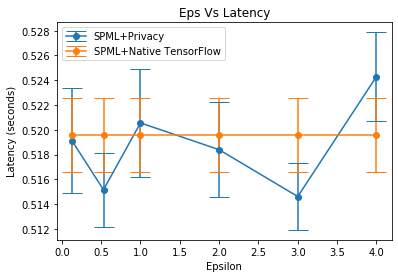
\includegraphics[width=\textwidth]{images/Inference/RRSIMLatency.png}
         \caption{Latency}
         \label{fig:simRRLatencyInference}
     \end{subfigure}
        \caption{Randomized response - Inference - Simulation mode without Intel SGX and with SCONE}
     \begin{subfigure}{0.5\textwidth}
         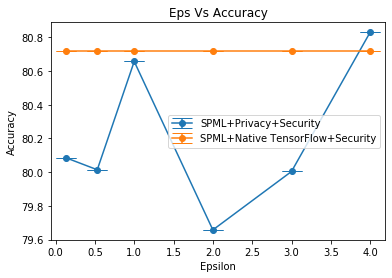
\includegraphics[width=\textwidth]{images/Inference/RRHWAccuracy.png}
         \caption{Accuracy}
         \label{fig:hwRRAccuracyInference}
     \end{subfigure}
     \begin{subfigure}{0.5\textwidth}
         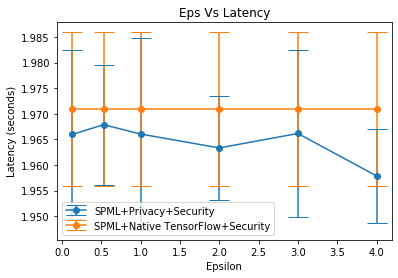
\includegraphics[width=\textwidth]{images/Inference/RRHWLatency.png}
         \caption{Latency}
         \label{fig:hwRRLatencyInference}
     \end{subfigure}
        \caption{Randomized response - Inference - Hardware mode with Intel SGX and SCONE}
\end{figure}
\newline
\newline
\textbf{\textit{Latency: }}We can see the latency values in Figure ~\ref{fig:nativeRRLatencyInference}, ~\ref{fig:simRRLatencyInference}, ~\ref{fig:hwRRLatencyInference} . SPML without privacy and SPML+privacy has the same latency of around 0.32 seconds for native mode. SPML has a latency of around 0.52 seconds for simulation mode while SPML + security is touching latency of around 1.95 seconds. After enabling security property in SPML latency is almost 6$\times$ as compared to SPML without security. Hence, the inference phase is much faster for our system SPML as compare to the training phase for randomized response also.

We have already seen MNIST and CIFAR10 dataset results already as well as randomized responses, in the discussion section ~\ref{sec:evalDiscussion}, we will summarize what we have learned from the measurements and what can be concluded about these runs and different modes. Before discussing the results, in the next section we have evaluated our system SPML against one of the machine learning attack to see visually the application of SPML.

\section{Machine learning attack}
\label{sec:evalMLAttack}
We also evaluated our system SPML against model inversion attack \cite{17} to proof our work. The model inversion attack as defined in \cite{17} states, if an adversary has access to a trained model and some auxiliary information about an individual, then it can make predictions about an individual’s genetic markers. This particular attack is discussed via an example from the pharmacogenetics field in the paper, but it can be generalized in any scenario like we have used this type of attack on the classification of hand-written digits from MNIST \cite{12} dataset.
\begin{figure}
     \begin{subfigure}{.325\textwidth}
         
\includegraphics[width=\textwidth]{images/Native_attack/Mnistattack_native.pdf}
         \vspace{-8em}
         \caption{SPML+Native TensorFlow; and, Accuracy=99.55\%}
         \label{fig:nativeEps0}
     \end{subfigure}
     \begin{subfigure}{.325\textwidth}
         \includegraphics[width=\textwidth]{images/Native_attack/Mnistattack.2.pdf}
         \vspace{-8em}
         \caption{SPML+Privacy; $\epsilon$=0.2; and, Accuracy=10.12\%;}
         \label{fig:nativeEps.2}
     \end{subfigure}
     \begin{subfigure}{.325\textwidth}
         \includegraphics[width=\textwidth]{images/Native_attack/Mnistattack8.pdf}
         \vspace{-8em}
         \caption{SPML+Privacy; $\epsilon$=8; and, Accuracy=85.36\%;}
         \label{fig:nativeEps8}
     \end{subfigure}
        \caption{Model inversion attack images - Native mode without Intel SGX and SCONE}
%\end{figure}
%\begin{figure}
     \begin{subfigure}{.325\textwidth}
         \includegraphics[width=\textwidth]{images/Sim_attack/Mnistattack_native.pdf}
         \vspace{-8em}
         \caption{SPML+Native TensorFlow; and, Accuracy=99.72\%}
         \label{fig:simEps0}
     \end{subfigure}
     \begin{subfigure}{.325\textwidth}
         \includegraphics[width=\textwidth]{images/Sim_attack/Mnistattack.2.pdf}
         \vspace{-8em}
         \caption{SPML+Privacy; $\epsilon$=0.2; and, Accuracy=11.66\%;}
         \label{fig:simEps.2}
     \end{subfigure}
     \begin{subfigure}{.325\textwidth}
         \includegraphics[width=\textwidth]{images/Sim_attack/Mnistattack8.pdf}
         \vspace{-8em}
         \caption{SPML+Privacy; $\epsilon$=8; and, Accuracy=84.37\%;}
         \label{fig:simEps8}
     \end{subfigure}
        \caption{Model inversion attack images - Simulation mode without Intel SGX and with SCONE}
%\end{figure}
%\begin{figure}
     \begin{subfigure}{.325\textwidth}
         \includegraphics[width=\textwidth]{images/Hw_attack/Mnistattack_native.pdf}
         \vspace{-8em}
         \caption{SPML+Native TensorFlow; and, Accuracy=99.65\%}
         \label{fig:hwEps0}
     \end{subfigure}
     \begin{subfigure}{.325\textwidth}
         \includegraphics[width=\textwidth]{images/Hw_attack/Mnistattack.2.pdf}
         \vspace{-8em}
         \caption{SPML+Privacy; $\epsilon$=0.2; and, Accuracy=10.19\%;}
         \label{fig:hwEps.2}
     \end{subfigure}
     \begin{subfigure}{.325\textwidth}
         \includegraphics[width=\textwidth]{images/Hw_attack/Mnistattack8.pdf}
         \vspace{-8em}
         \caption{SPML+Privacy; $\epsilon$=8; and, Accuracy=85.93\%;}
         \label{fig:hwEps8}
     \end{subfigure}
        \caption{Model inversion attack images - Hardware mode with Intel SGX and SCONE}
\end{figure}
To implement this attack \footnote{https://github.com/prbh695a/SPML/tree/master/Model\%20Inversion\%20attack}, we have used IBM's open-source Adversarial Robustness Toolbox (ART) \cite{76} library. The model is trained with the MNIST dataset with 60,000 training samples. We have used 10,000 test samples as explained in the library for better visualization. We have assumed the mean values of test data for each digit as the auxiliary information for our evaluation. We used epsilon values as 0.2, 1, 2, 4, 6, 8 in all three modes which are native mode (i.e without Intel SGX and SCONE), SCONE simulation mode, and SCONE hardware mode.

In all the modes (i.e native, SCONE simulation, and SCONE hardware), the attack is executed on SPML+Native TensorFlow and SPML+Privacy. We enable privacy property in all three modes, and security property is enabled in SCONE hardware mode only. When the attack was done on the SPML+Native TensorFlow trained model, we can see that in Figure ~\ref{fig:nativeEps0}, ~\ref{fig:simEps0}, ~\ref{fig:hwEps0}, that many of the digits are revealed and we can take hints what kind of training data was used. Hence, our attack is successful. Therefore, without enabling privacy property individual training data is leaked. SPML aims to protect individual's information by enabling privacy property to prevent such types of attacks.

The privacy property is enabled for different epsilon values as 0.2, 1, 2, 4, 6, 8. For the discussion purpose, we will be discussing epsilon values 0.2 and 8 only, as the rest of the epsilon values showed almost the same results. However, for completeness, the detailed images for all the trained models with different epsilon values are shown in ~\ref{sec:MIA}. When the attack was executed on the model trained with epsilon value 8 with our system SPML, as shown in Figure ~\ref{fig:nativeEps8}, ~\ref{fig:simEps8}, ~\ref{fig:hwEps8} then we are not able to make out any of the images used in the training set.  The trained model with epsilon value 8 has an accuracy of almost 85 percent but still, we cannot visualize the images clearly because we have enabled privacy property in our system SPML.

The model trained with epsilon value from 0.2 to 4 achieved an accuracy of around 10-11\% hence these models cannot be used for classification in practice. Visually also, the images are not usable as shown in Figure ~\ref{fig:nativeEps.2}, ~\ref{fig:simEps.2}, ~\ref{fig:hwEps.2}. Hence, the privacy property and accuracy have a trade-off which we should make. The trade-off can be seen graphically and mathematically in sections ~\ref{sec:evalMnist} and ~\ref{sec:evalCifar10} and this section proves this trade-off visually. 

We can conclude that our system SPML not only protects the confidentiality and integrity of the system but it also avoids leakage of private and sensitive information of the individuals participating in the training dataset. 

\section{Discussion}
\label{sec:evalDiscussion}
In this section, we will discuss how our system SPML system performed in terms of accuracy and latency. We will be using the measurement from the MNIST, CIFAR10 dataset as seen above. This section is divided into two parts to study the effect of (1) Privacy (2) Confidentiality and integrity property. Privacy is achieved using differential privacy which is implemented using TensorFlow privacy library \cite{11} or randomized response. Confidentiality and integrity are achieved using Intel SGX and integration is done using SCONE runtime environment. We will first discuss the effect of enabling only privacy and then the effect of enabling both privacy and security in our system SPML with noise and in the next subsection we will discuss randomized response separately.

\subsection{Privacy:} 
When privacy is added to the data, we aim to protect the individual's information from any kind of leakage that could happen via attacks as discussed in the background chapter ~\ref{sec:attackOnML}. To implement privacy, we are using the TensorFlow privacy library which uses differential privacy techniques to add privacy. In this library, random Gaussian noise is added during the training of the model.
\newline
\newline
\textbf{\textit{Training phase: }}For the training phase, when we add only privacy to the system the accuracy increases with epsilon value as seen in Figure ~\ref{fig:nativeMnistAccuracyTraining}. However, latency for DP(SPML+privacy) run is almost 10$\times$ higher than the native TensorFlow(SPML) run for MNIST as shown in ~\ref{fig:nativeMnistLatencyTraining}. This is the cost of adding privacy in our system SPML. One has to bear this cost if the privacy-preserving system is needed using the TensorFlow privacy library.
\newline
\newline
\textbf{\textit{Inference phase: }}On the other hand if we look at the results of the inference phase, then accuracy holds the same notion as discussed above, which is accuracy increases with epsilon value as seen in Figure ~\ref{fig:nativeMnistAccuracyInference}. The latency of the inference phase is almost the same for both runs i.e with and without privacy. This is one of the advantages of our system, that inference latency is not affected by the addition of privacy. In terms of productivity, we can say that once the model is trained, an inference can be done in normal working hours with no or very less wait times, however training should be planned in advance due to high training time. After discussing privacy property, we want to discuss security property affect on SPML.

\subsection{Confidentiality and Integrity}
When we add confidentiality and integrity to an application/system we have to use encryption and decryption. This means data, code, and model will be in encrypted form and before executing in an enclave this will be decrypted. The same thing is applicable for the output, it will be decrypted inside an enclave and will be encrypted when it will be saved on the disk (outside an enclave). This encryption/decryption will be adding additional overhead for any system/application where confidentiality and integrity have to be added. We have used the SCONE runtime environment which enables us to use TEEs easily and transparently. For TEEs, we have used Intel SGX for our system SPML. We will first discuss the training phase and then the inference phase for accuracy and latency for SPML.
\newline
\newline
\textbf{\textit{Training phase: }}For the training phase, accuracy is not affected a lot when we add confidentiality and integrity to the data, code, and model as seen in Figure ~\ref{fig:hwMnistAccuracyTraining}. The accuracy is affected only by enabling privacy property as discussed above, enabling security property is not affecting accuracy. It remains almost comparable to native and simulation mode for both the native TensorFlow (SPML+native TensorFlow) and DP runs (SPML+privacy). However, latency, as expected, degraded a lot after enabling security property. In the hardware mode, the native TensorFlow (SPML+security) run has a latency of almost 10$\times$ as compared to native mode (SPML). On the other hand, DP (SPML+security+privacy) runs have a latency of almost 25$\times$ as compared to native (SPML+privacy) mode. Hence, it's not possible to train models in working hours, we have to plan nightly or weekend runs for training the models after enabling security and privacy property.
\newline
\newline
\textbf{\textit{Inference phase: }}For the inference phase, the accuracy trend remains same as discussed above in the training phase. The security property is not affecting accuracy. The latency remains the same for native TensorFlow(SPML+security) and DP(SPML+privacy+security) run in hardware mode. For hardware mode (SPML+security+privacy) latency is 6$\times$ times  than the native mode (SPML+privacy). Inference latency is within the acceptable limit and hence can be used in practice. 

We can conclude that privacy property is affecting both the evaluation parameters which is accuracy and latency for SPML. At the strong privacy bounds which is at low epsilon values, the accuracy is very low and at weaker privacy bounds which is at higher epsilon values accuracy is acceptable. As seen, from the figures of the attack ~\ref{fig:nativeEps0}, ~\ref{fig:nativeEps.2} and ~\ref{fig:nativeEps8}, models trained with high epsilon values can be used in practice and they provide privacy also. The is the trade off we have discussed between the privacy and accuracy level. It is left to the individual how they want to apply this trade off in their respective applications or systems. On the other hand, security property only affects latency parameter. Accuracy is independent of security property. Hence we can control the accuracy level in SPML according to our requirement. Therefore, if we enable both the properties in SPML, then we have to pay the cost of enabling these properties in terms of only latency and to an extent accuracy and we get important properties like privacy, confidentiality and integrity.

\subsection{Randomized response}
The advantage of using randomized noise is that each user can make their data differentially private while filling up the responses for the survey or during data collection. It enables the user to have plausible deniability. However, when it is used on the training dataset, though it makes models differentially private, another parameter such as accuracy is hard to depict. Sometime it may result in better accuracy than a native algorithm or sometimes worse as seen in the above Figures ~\ref{fig:nativeRRAccuracyTraining}, ~\ref{fig:simRRAccuracyTraining} and ~\ref{fig:hwRRAccuracyTraining}. This is because the datapoint in data can be changed as a whole which makes the dataset entirely different. After looking above measurement we can conclude that no trend can be exactly said for accuracy and epsilon values, however, latency is not affected much by enabling privacy property it remains the same. Latency is deteriorated 4.2$\times$, 5.2$\times$ for training and inference phase respectively for enabling security property as compare to without security property. Hence, in practice, we can use inference as well as training for this type of technique. However, we need a way to make it more generalize as it can be only applied to statistical survey techniques for making predictions. For classification problems (image or object), it may need more work. 

Hence, it is better to use SPML and achieve differential privacy with noise as it can be used to predict as well as classify and very few changes are required in the existing system. There is a clear trend for accuracy and we have more control over how much noise should be added as opposed to a randomized response where it is hard to establish a clear trend between accuracy and epsilon value. SPML system takes more time for training as compared to inference and hence training should be planned well in advance either for nightly or weekend run. On the other hand, inference can be done in practice with fewer wait times. It is easy to use our system for training the models and inference anytime. There are very minimal code changes require to add privacy and security properties. Next, we will discuss some advance features of SPML so that training can also be used in practise.
%\cleardoublepage

\section{Advance Features}
SPML system only cost we have to pay is in terms of latency, so if somehow we can improve the latency of the SPML then it will make our system more efficient. In this section, we will be discussing some more advanced features that we have tried to improve the efficiency of the system.

\subsection{Inference only in SCONE hardware mode}
\label{sec:ioonly}
The first feature to reduce the latency in hardware mode is to use only inference in hardware mode. We can train a model in the native mode with only privacy property enabled. Once we have got the trained model we can encrypt it and use it for doing only inference in SCONE hardware mode. This will save a lot of our time. We ran only inference on the encrypted previously trained model and results are almost the same as doing inference in native mode. The plots are available in Appendix section ~\ref{sec:appIO}.

\subsection{Training model in native and hardware mode}
The second feature is to train the model on some already available samples in native mode and later continue the training in hardware mode with new samples. It means that we will be providing more training samples on an already trained model. Therefore, we will be saving time from training the model from the scratch. We call this approach as 'save and load model'. \newline
\newline
\textbf{\textit{Save and load model: }}
\label{sec:workaroundSLmodel}
We can simply train the model using the available samples until the last epoch and save that model. Later deploy the encrypted model in SCONE hardware mode, decrypt it, and continue training over it. In this way, the model needs to be trained only for a new sample which can be done in less time as compared to training the whole model from scratch. To conclude how it works in practice, we split the MNIST dataset into two halves. The first half is trained in native mode and later we trained second half in hardware mode. When we plotted the graphs for this run we got almost comparable results as discussed in appendix section \ref{sec:appNHmode}. However, if during the training if there is a way to pick up the best trained model or to stop training early if accuracy is not improving further then it will further reduce the training time. It is possible to achieve both of these approaches using 'checkpointing' and 'earlystopping'.

\subsubsection{Checkpointing the best model}
The approach is based on the previously discussed technique of 'save and load model' \ref{sec:workaroundSLmodel}. The Keras \cite{83} library provide a way to checkpoint the best trained model using \textit{ModelCheckpoint} API \cite{84}. This way we can train the best model in native mode and checkpoint it \footnote{https://github.com/prbh695a/SPML/blob/master/Noise/MNIST/CheckPointing/bestmodel.py}. Later we can use the encrypted check-pointed model, deploy it in SCONE hardware mode to do inference, or may further train it. This way we can improve accuracy further by working with the best trained model always. In this approach, the training will take place until the end of all the epochs and only way to reduce latency is to train model with maximum sample in the native mode first and then deploy in hardware mode to do inference or training further. This approach will definitely provide the best accuracy model but we gain little on the latency reduction hence we tried one more approach known as 'earlystopping'.

\subsubsection{Earlystopping}
The next approach we tried is early stopping \cite{85}. We can monitor some metrics for example 'accuracy' and can stop training once it has stopped to improve further \footnote{https://github.com/prbh695a/SPML/blob/master/Noise/MNIST/CheckPointing/earlystopping.py}. For example, during the model training, the accuracy can be checked after each iteration(i.e epoch), and training is stopped if it's not increasing further by specifying the patience level. Using this technique we don't have to wait until the end of all epochs, training can be stopped if monitored metrics (i.e accuracy in our example) is not improving further. This approach reduces training time in any mode and hence can reduce latency. We have seen that trained model can be saved and used later on for inference or to continue the training further. 

We ran the early-stopping measurements on the MNIST dataset. We trained the model by enabling early stopping in hardware mode. In the figure ~\ref{fig:EsMnistAccuracyTraining} and ~\ref{fig:EsMnistLatencyTraining} we compared the result of early-stopping training vs training without early-stopping. We can observe that training accuracy is comparable for every epsilon value and latency is reduced from 775 seconds to around 485 seconds. Hence, we are getting a gain of almost 1.5$\times$ by using early-stopping.

\begin{figure}
     \begin{subfigure}{0.5\textwidth}
         \includegraphics[width=\textwidth]{images/Training/MnistESAccuracy.png}
         \caption{Accuracy}
         \label{fig:EsMnistAccuracyTraining}
     \end{subfigure}
     \begin{subfigure}{0.5\textwidth}
         \includegraphics[width=\textwidth]{images/Training/MnistESLatency.png}
         \caption{Latency}
         \label{fig:EsMnistLatencyTraining}
     \end{subfigure}
        \caption{MNIST Dataset - Training - Earlystopping}
\end{figure}

As a continuation in the recent research, a distributed machine learning approach known as Federated learning \cite{86} is gaining lot of attention. In brief, it states that we don't need to share the sensitive and private data always instead we can just share the trained model. Then we can average out the model parameters of various trained model and in few rounds we will get good amount of accuracy without sharing the private and sensitive training data and hence data privacy can be preserved. We also explored this approach by running a small experiment on federated learning.

\subsection{Federated learning}
\label{sec:flTEE}
Till now we have seen the standard machine learning approaches wherein the training data is centralized and kept at one machine or data center. There are few issues with this approach such as if an attacker can breach the security of the data center then it may get hold of the whole training data. Another issue is that in small devices like mobile phones, the computation resources are limited therefore they cannot train the model on the whole training data. We need some way to decentralized the data and simultaneously reap the benefit of machine learning. This problem is solved by using Federated learning \cite{86}.

\begin{figure}[h!]
    \centering
    \includegraphics[width=10cm, height=10cm]{images/FL.pdf}
    \caption{Federated Learning}
    \label{fig:fld}
\end{figure}

Federated learning introduces a decentralized approach for machine learning. As show in Figure ~\ref{fig:fld}, in this approach, each device/user train the model with its local data and then send this trained local model to the server. The server aggregates the locally trained model from many devices to produce a final aggregate or global model. The server then sends the aggregate/global model for further training from each user's local data. In this way, the local data of the user is never shared, and only a trained local model and aggregate trained model is exchanged in every round of client-server communication. After a few rounds, the aggregate model will get good accuracy without even having actual training data and hence privacy of the user data is preserved as it is never shared.

\begin{table}[h!]
\begin{center}
\caption{Federated Learning Rounds - Accuracy in \%}
\label{tab:flrounds}
\begin{tabular}{|c|c|c|c|c|c|}
\hline
Rounds & Client1 & Client2 & Client3 & Client4 & Server \\
\hline
1      & 15.48   & 28.88   & 27.56   & 15.24   & 10.88  \\
\hline
2      & 33.96   & 31.28   & 21.52   & 22.16   & 27.2   \\
\hline
3      & 9       & 49.6    & 48.72   & 22.28   & 22.64  \\
\hline
4      & 72.48   & 58.92   & 77.68   & 66.28   & 69.72  \\
\hline
5      & 78.44   & 82.64   & 82.68   & 80.64   & 86.04  \\
\hline
6      & 89      & 85.68   & 89.8    & 89.2    & 89.8   \\
\hline
7      & 85.76   & 81.52   & 80.8    & 90.44   & 90.68  \\
\hline
8      & 92.04   & 89.04   & 90.56   & 91.52   & 92.4   \\
\hline
9      & 92.56   & 87.72   & 81.6    & 90.92   & 91.52  \\
\hline
10     & 92.28   & 92.64   & 93.36   & 92.48   & 93.48  \\
\hline
\end{tabular}
\end{center}
\end{table}

We tried this approach on the MNIST dataset \footnote{https://github.com/prbh695a/SPML/tree/master/Noise/MNIST/FL}. We split MNIST dataset into 4 parts, each part training 2500 samples. Then, we aggregated or averaged the model parameters of all these parts to produce an aggregate model. We call these parts as 'Client1', 'Client2', 'Client3' and 'Client4'. Clients are trained in native mode which can be on small individual devices (such as mobile phone), while aggregation is done on server using Intel SGX (hardware mode). 

We used test data of 2500 samples on the final aggregate model. As shown in table ~\ref{tab:flrounds}, in round-1 the aggregate model shows test accuracy of around 10.88\% and in round-10 the aggregate model started showing an accuracy of around 93.48\%. In this approach we simulated a scenario wherein we train the aggregate model in the SCONE hardware mode, while local training happened on each individual user's device (native mode) to reduce latency further.

\chapter{Future work}
\label{sec:fw}
In this chapter, we will focus on future work and improvements that can be done over our existing system. SPML system is a prototype that shows we can achieve privacy, confidentiality, and integrity on any native machine/deep learning system. To make our system production-ready, we still need to put some more efforts like we have to integrate more modules of SCONE, add a generalized random response mechanism, explore Laplace noise. We want to discuss a few of the future work and improvements as follows:

\section{SCONE CAS}
In the current prototype, we have used the system without the SCONE CAS \cite{78}  module. When deploying in production, SCONE CAS (Configuration and Attestation Service) is used for service attestation and policy management. It is the main module that can attest to all the enclaves in the network. But due to time limitations, we have focused only on the integral parts of the system. We have concentrated on making a generic machine learning framework SPML, that will provide privacy, confidentiality, and integrity to any existing native machine learning application. Hence, integration with SCONE CAS is needed to make the SPML system production-ready.

\section{Generalized randomized response}
In the current SPML prototype, we have shown that a randomized response technique, based on coin flips, can also be used to add privacy to the system. There are many other ways to implement randomized responses such as proposed in Google's RAPPOR paper \cite{5} or algorithms suggested by Apple \cite{75} such as Private Count Mean Sketch, Private Hadamard Count Mean Sketch, Private Sequence Fragment Puzzle. As an enhancement, these techniques can also be studied with our system SPML.

\section{Laplace noise}
In the current SPML prototype, we have used the DP library based on paper \cite{4} and implemented privacy property with Gaussian noise. The privacy library also provides an option to add Laplace noise based on 'Bolt-on Differential Privacy' \cite{79}. In practice, Laplace's noise is more practical than Gaussian noise. Hence, we can evaluate our system SPML with Laplace noise to study its effects in the future.

\section{Implementation with other frameworks}
In the current SPML, we have used Google's open-source framework TensorFlow \cite{24}. As an enhancement, we can make SPML more generic by implementing using Pytorch \cite{75} also. Pytorch is also an emerging and promising open-source framework used industry-wide.

\chapter{Conclusion}
\label{sec:conclusion}
In this thesis, we have created a secure privacy-preserving machine learning framework SPML that enforces privacy, confidentiality, and integrity on any native machine/deep learning system. We have developed this framework with the help of Google TensorFlow \cite{24}, differential privacy library \cite{11}, or randomized response to achieve privacy, Intel SGX \cite{9} to achieve security goals of confidentiality and integrity and SCONE \cite{22} for integration with TEEs. We have used the SCONE platform so that native and legacy systems can use SPML with minimum code changes.

Privacy property is achieved by adding noise or randomized response and for enabling security property we have used Intel SGX. For noise, SPML shows a trend for the accuracy upon enabling privacy property, which is accuracy increases with epsilon value and this trend remains unaffected upon enabling security property for both the training and inference phase. The latency however increases upon enabling privacy and security property for the training phase. On the other hand, the inference phase for SPML can be completed within a few seconds upon enabling these properties. 

The latency for the randomized response mechanism is less as compared to using a noise mechanism. However, accuracy for randomized response fluctuates a lot which makes it less useful in practice. On the other hand, due to the notion that we saw for noise between the accuracy and epsilon values in the evaluation section ~\ref{sec:eval}, which is accuracy increases with epsilon values, using noise is much more practical as compared to the randomized response. 

It can be concluded that the SPML system is practical to use for inference but for training, it takes more time. If we have to make our native machine learning system privacy-preserving and secure then we have to bear this cost in terms of latency in both the mechanisms i.e randomized response or noise. We can use some of the advanced features to deploy the system and reduce training time further such as 'Inference only in SCONE hardware mode' ~\ref{sec:ioonly}, 'Save and load model' ~\ref{sec:workaroundSLmodel} or 'federated learning' ~\ref{sec:flTEE} as discussed in the evaluation chapter.

Our system SPML, not only makes any native existing machine/deep learning system privacy-preserving but it also provides confidentiality and integrity using Intel SGX. We have used the SCONE runtime environment to wrap up the integration with TEEs and SCONE being a container-based environment makes SPML easy to deploy, run, and maintain in native or cloud environments. SPML is not only easy to use for new developments but any existing native machine learning system can use our system SPML framework and with minimum code changes privacy and security properties can be added in these native machine learning systems.

\clearpage
\appendix
\chapter{Appendix}
\section{Model inversion attack - images}
\label{sec:MIA}
In section ~\ref{sec:attackOnML}, we have discussed about the model inversion attack on machine learning systems. We showed images only for native Tensorflow trained model, and differentially private model with epsilon values 0.2 and 8 in section 6.5. The complete images we got from trained model with different epsilon values are shown in Figure A.1, A.2 and A.3.
\begin{figure}[h!]
     \begin{subfigure}{.325\textwidth}
         \includegraphics[width=\textwidth]{images/Native_attack/Mnistattack_native.pdf}
         \vspace{-8em}
         \caption{SPML+Native TensorFlow; and, Accuracy=99.55\%}
         \label{default}
     \end{subfigure}
     \begin{subfigure}{.325\textwidth}
         \includegraphics[width=\textwidth]{images/Native_attack/Mnistattack.2.pdf}
         \vspace{-8em}
         \caption{SPML+Privacy; $\epsilon$=0.2; and, Accuracy=10.12\%}
         \label{default}
     \end{subfigure}
     \begin{subfigure}{.325\textwidth}
         \includegraphics[width=\textwidth]{images/Native_attack/Mnistattack1.pdf}
         \vspace{-8em}
         \caption{SPML+Privacy; $\epsilon$=1 ; and, Accuracy=10.91\%}
         \label{default}
     \end{subfigure}
     \begin{subfigure}{.325\textwidth}
         \includegraphics[width=\textwidth]{images/Native_attack/Mnistattack2.pdf}
         \vspace{-8em}
         \caption{SPML+Privacy; $\epsilon$=2 ; and, Accuracy=10.63\%}
         \label{default}
     \end{subfigure}
     \begin{subfigure}{.325\textwidth}
         \includegraphics[width=\textwidth]{images/Native_attack/Mnistattack4.pdf}
         \vspace{-8em}
         \caption{SPML+Privacy; $\epsilon$=4 ; and, Accuracy=66.3\%}
         \label{default}
     \end{subfigure}
     \begin{subfigure}{.325\textwidth}
         \includegraphics[width=\textwidth]{images/Native_attack/Mnistattack6.pdf}
         \vspace{-8em}
         \caption{SPML+Privacy; $\epsilon$=6 ; and, Accuracy=80.19\%}
         \label{default}
     \end{subfigure}
     \begin{subfigure}{.325\textwidth}
         \includegraphics[width=\textwidth]{images/Native_attack/Mnistattack8.pdf}
         \vspace{-8em}
         \caption{SPML+Privacy; $\epsilon$=8 ; and, Accuracy=85.36\%}
         \label{default}
     \end{subfigure}
        \caption{Model inversion attack images - Native mode without Intel SGX and SCONE}
        \label{default}
\end{figure}

\begin{figure}
     \begin{subfigure}{.325\textwidth}
         \includegraphics[width=\textwidth]{images/Sim_attack/Mnistattack_native.pdf}
         \vspace{-8em}
         \caption{SPML+Native TensorFlow; and, accuracy=99.72\%}
         \label{default}
     \end{subfigure}
     \begin{subfigure}{.325\textwidth}
         \includegraphics[width=\textwidth]{images/Sim_attack/Mnistattack.2.pdf}
         \vspace{-8em}
         \caption{SPML+Privacy; $\epsilon$=0.2; and, Accuracy=11.66\%}
         \label{default}
     \end{subfigure}
     \begin{subfigure}{.325\textwidth}
         \includegraphics[width=\textwidth]{images/Sim_attack/Mnistattack1.pdf}
         \vspace{-8em}
         \caption{SPML+Privacy; $\epsilon$=1; and, Accuracy=10.07\%}
         \label{default}
     \end{subfigure}
     \begin{subfigure}{.325\textwidth}
         \includegraphics[width=\textwidth]{images/Sim_attack/Mnistattack2.pdf}
         \vspace{-8em}
         \caption{SPML+Privacy; $\epsilon$=2; and, Accuracy=10.54\%}
         \label{default}
     \end{subfigure}
     \begin{subfigure}{.325\textwidth}
         \includegraphics[width=\textwidth]{images/Sim_attack/Mnistattack4.pdf}
         \vspace{-8em}
         \caption{SPML+Privacy; $\epsilon$=4; and, Accuracy=67.76\%}
         \label{default}
     \end{subfigure}
     \begin{subfigure}{.325\textwidth}
         \includegraphics[width=\textwidth]{images/Sim_attack/Mnistattack6.pdf}
         \vspace{-8em}
         \caption{SPML+Privacy; $\epsilon$=6; and, Accuracy=71.6\%}
         \label{default}
     \end{subfigure}
     \begin{subfigure}{.325\textwidth}
         \includegraphics[width=\textwidth]{images/Sim_attack/Mnistattack8.pdf}
         \vspace{-8em}
         \caption{SPML+Privacy; $\epsilon$=8; and, Accuracy=84.37\%}
         \label{default}
     \end{subfigure}
        \caption{Model inversion attack images - SCONE simulation mode without Intel SGX and with SCONE}
        \label{default}
\end{figure}

\begin{figure}
     \begin{subfigure}{.325\textwidth}
         \includegraphics[width=\textwidth]{images/Hw_attack/Mnistattack_native.pdf}
         \vspace{-8em}
         \caption{SPML+Native TensorFlow; and, accuracy=99.65\%}
         \label{default}
     \end{subfigure}
     \begin{subfigure}{.325\textwidth}
         \includegraphics[width=\textwidth]{images/Hw_attack/Mnistattack.2.pdf}
         \vspace{-8em}
         \caption{SPML+Privacy; $\epsilon$=0.2; and, Accuracy=10.19\%}
         \label{default}
     \end{subfigure}
     \begin{subfigure}{.325\textwidth}
         \includegraphics[width=\textwidth]{images/Hw_attack/Mnistattack1.pdf}
         \vspace{-8em}
         \caption{SPML+Privacy; $\epsilon$=1; and, Accuracy=10.13\%}
         \label{default}
     \end{subfigure}
     \begin{subfigure}{.325\textwidth}
         \includegraphics[width=\textwidth]{images/Hw_attack/Mnistattack2.pdf}
         \vspace{-8em}
         \caption{SPML+Privacy; $\epsilon$=2; and, Accuracy=10.39\%}
         \label{default}
     \end{subfigure}
     \begin{subfigure}{.325\textwidth}
         \includegraphics[width=\textwidth]{images/Hw_attack/Mnistattack4.pdf}
         \vspace{-8em}
         \caption{SPML+Privacy; $\epsilon$=4; and, Accuracy=53.13\%}
         \label{default}
     \end{subfigure}
     \begin{subfigure}{.325\textwidth}
         \includegraphics[width=\textwidth]{images/Hw_attack/Mnistattack6.pdf}
         \vspace{-8em}
         \caption{SPML+Privacy; $\epsilon$=6; and, Accuracy=75.92\%}
         \label{default}
     \end{subfigure}
     \begin{subfigure}{.325\textwidth}
         \includegraphics[width=\textwidth]{images/Hw_attack/Mnistattack8.pdf}
         \vspace{-8em}
         \caption{SPML+Privacy; $\epsilon$=8; and, Accuracy=85.93\%}
         \label{default}
     \end{subfigure}
        \caption{Model inversion attack images - SCONE hardware mode with Intel SGX and with SCONE}
        \label{default}
\end{figure}
\clearpage
\section{Advanced feature}
In the evaluation section ~\ref{sec:eval}, we have seen that training the model takes a lot of time while inference is fast. To overcome this problem, we tried some advance feature such as (1) Inference with previously saved model (2) Save and load model

\subsection{Inference with previously saved model}
\label{sec:appIO}
We can train the model with SPML+privacy in native mode (without Intel SGX and SCONE). In this mode, training time is very less (around 30 seconds) for the MNIST dataset as compare to SPML+privacy+security mode (around 775 seconds), which will save a lot of the time. The model which we have got can be used for doing inference in SCONE hardware mode with security property enabled. We ran some measurements wherein we use the model trained in native mode and deploy the model in SCONE hardware mode to check the impact. As seen in the Figure  ~\ref{fig:appendixPSMnistAccuracyInference} and ~\ref{fig:appendixPSMnistLatencyInference}, the accuracy and latency remains almost same as compare to native mode ~\ref{fig:appendixnativeMnistAccuracyInference} and ~\ref{fig:appendixnativeMnistLatencyInference} and the hardware mode ~\ref{fig:appendixhwMnistAccuracyInference} and ~\ref{fig:appendixhwMnistLatencyInference}.

\subsection{Save and load model}
\label{sec:appNHmode}
We can train the model with some samples in SPML+privacy in native mode (without Intel SGX and SCONE) and later load the saved model and continue training in hardware mode. This type of technique is used in federated learning also where in each individual device train models using local data in a decentralized way, and then send this trained model to central server which combines resultant model to generate a global model. We can opt for such approach to reduce training time.
As seen in the Figure ~\ref{fig:appendixFLMnistAccuracyInference},  ~\ref{fig:appendixFLMnistLatencyInference} the accuracy and latency remains almost same as compare to native ~\ref{fig:appendixnativeMnistAccuracyInference} and ~\ref{fig:appendixnativeMnistLatencyInference}, and the hardware mode ~\ref{fig:appendixhwMnistAccuracyInference} and ~\ref{fig:appendixhwMnistLatencyInference}

\begin{figure}
     \begin{subfigure}{0.5\textwidth}
         \includegraphics[width=\textwidth]{images/Inference/MnistNativeAccuracyInference.png}
         \caption{Accuracy}
         \label{fig:appendixnativeMnistAccuracyInference}
     \end{subfigure}
     \begin{subfigure}{0.5\textwidth}
         \includegraphics[width=\textwidth]{images/Inference/MnistNativeLatencyInference.png}
         \caption{Latency}
         \label{fig:appendixnativeMnistLatencyInference}
     \end{subfigure}
        \caption{MNIST Dataset - Inference - Native mode without Intel SGX and SCONE}
     \begin{subfigure}{0.5\textwidth}
         \includegraphics[width=\textwidth]{images/Inference/MnistHwAccuracyInference.png}
         \caption{Accuracy}
         \label{fig:appendixhwMnistAccuracyInference}
     \end{subfigure}
     \begin{subfigure}{0.5\textwidth}
         \includegraphics[width=\textwidth]{images/Inference/MnistHwLatencyInference.png}
         \caption{Latency}
         \label{fig:appendixhwMnistLatencyInference}
     \end{subfigure}
        \caption{MNIST Dataset - Inference - Hardware mode with Intel SGX and SCONE}
     \begin{subfigure}{0.5\textwidth}
         \includegraphics[width=\textwidth]{images/Inference/MnistPSAccuracyInference.png}
         \caption{Accuracy}
         \label{fig:appendixPSMnistAccuracyInference}
     \end{subfigure}
     \begin{subfigure}{0.5\textwidth}
         \includegraphics[width=\textwidth]{images/Inference/MnistPSLatencyInference.png}
         \caption{Latency}
         \label{fig:appendixPSMnistLatencyInference}
     \end{subfigure}
        \caption{MNIST Dataset - Inference+Saved Model - Hardware mode + Fspf with Intel SGX and SCONE}
\end{figure}


\begin{figure}
     \begin{subfigure}{0.5\textwidth}
         \includegraphics[width=\textwidth]{images/Training/MnistFLAccuracy.png}
         \caption{Accuracy}
         \label{fig:appendixFLMnistAccuracyTraining}
     \end{subfigure}
     \begin{subfigure}{0.5\textwidth}
         \includegraphics[width=\textwidth]{images/Training/MnistFLLatency.png}
         \caption{Latency}
         \label{fig:appendixFLMnistLatencyTraining}
     \end{subfigure}
        \caption{MNIST Dataset - training - native+hardware Mode - Hardware mode + Fspf with Intel SGX and SCONE}
     \begin{subfigure}{0.5\textwidth}
         \includegraphics[width=\textwidth]{images/Inference/MnistFLAccuracyInference.png}
         \caption{Accuracy}
         \label{fig:appendixFLMnistAccuracyInference}
     \end{subfigure}
     \begin{subfigure}{0.5\textwidth}
         \includegraphics[width=\textwidth]{images/Inference/MnistFLLatencyInference.png}
         \caption{Latency}
         \label{fig:appendixFLMnistLatencyInference}
     \end{subfigure}
        \caption{MNIST Dataset - inference - native+hardware Mode - Hardware mode + Fspf with Intel SGX and SCONE}
\end{figure}



\printbibliography
\end{document}
